\documentclass{beamer}
\usepackage{default}
\usepackage{amsmath}
\usepackage{graphicx}
\usepackage{adjustbox}  % Allows for fitting tables into slide
\usepackage{hyperref}
\usepackage{threeparttable}
\usepackage{caption}
%\usepackage{subcaption}
\usepackage{natbib}
\usepackage{adjustbox}
\usepackage{subcaption}
%\usetheme{AnnArbor}
%\usetheme{Antibes}
%\usetheme{Bergen}
%\usetheme{Berkeley}
%\usetheme{Berlin}
\usetheme{Boadilla}
%\usetheme{boxes}
%\usetheme{CambridgeUS}
%\usetheme{Copenhagen}
%\usetheme{Darmstadt}
%\usetheme{default}
%\usetheme{Frankfurt}
%\usetheme{Goettingen}
%\usetheme{Hannover}
%\usetheme{Ilmenau}
%\usetheme{JuanLesPins}
%\usetheme{Luebeck}
%\usetheme{Madrid}
%\usetheme{Malmoe}
%\usetheme{Marburg}
%\usetheme{Montpellier}
%\usetheme{PaloAlto}
%\usetheme{Pittsburgh}
%\usetheme{Rochester}
%\usetheme{Singapore}
%\usetheme{Szeged}
%\usetheme{Warsaw}

\title{Rigidity of Expectations: Additional Evidence from Density Forecasts of Professionals and Households}


% A subtitle is optional and this may be deleted

\author{Tao Wang \\ Johns Hopkins University}
% - Give the names in the same order as the appear in the paper.
% - Use the \inst{?} command only if the authors have different
%   affiliation.

\date{\today}
% - Either use conference name or its abbreviation.
% - Not really informative to the audience, more for people (including
%   yourself) who are reading the slides online

% This is only inserted into the PDF information catalog. Can be left
% out. 

% If you have a file called "university-logo-filename.xxx", where xxx
% is a graphic format that can be processed by latex or pdflatex,
% resp., then you can add a logo as follows:

% \pgfdeclareimage[height=0.5cm]{university-logo}{university-logo-filename}
% \logo{\pgfuseimage{university-logo}}

% Delete this, if you do not want the table of contents to pop up at
% the beginning of each subsection:
\AtBeginSubsection[]
{
	\begin{frame}<beamer>{Outline}
	\tableofcontents[currentsection]
\end{frame}
}

\begin{document}
	

\begin{frame}
	\titlepage
\end{frame}
\begin{frame}{Outline}
	\tableofcontents
	% You might wish to add the option [pausesections]
\end{frame}


\section{Motivation}

\begin{frame}{Motivation}
	\begin{itemize}
		\item there are various theories on  ``irrational expectation''
		\item different theories can be tested using survey data  in a comparable manner  (\citet{coibion2012can})
		\item a good theory needs to be (relatively) consistent in predictions across different moments
		\item higher moments, i.e. uncertainty, brings about one more restriction
		\item survey also contains information about data generating process itself
	\end{itemize}
\end{frame}


\begin{frame}{What this paper does}
	\begin{enumerate}
		\item time series and cross-sectional pattern of \textcolor{blue}{uncertainty} from \textbf{density} forecasts of the inflation 
		\item additional reduced-form tests of the full-information rationality null using the uncertainty 
		\item extend \citet{coibion2012can} in two ways 
		\begin{itemize}
		\item cross-moment estimation for each one of the particular theories on expectation 
		\item allowing for stochastic volatility of inflation process 
		\end{itemize}
	\end{enumerate}
\end{frame}


\begin{frame}{Literature}
\begin{itemize}
	\item empirical tests on expectation formation
	\begin{itemize}
		\item \citet{mankiw2003disagreement}, \citet{carroll2003macroeconomic}, \citet{branch2004theory}, \citet{malmendier2015learning}, \citet{das2017socioeconomic}, \citet{coibion2012can}, \citet{fuhrer2018intrinsic} 
	\end{itemize}
    \item density and probabilistic questions in expectation surveys
    \begin{itemize}
    	\item  \citet{manski2004measuring}, \citet{delavande2011measuring}, \citet{manski2018survey} 
    	\item  \citet{bertrand2001people},  \citet{van2008rethinking},  \citet{delavande2014probabilistic}
    \end{itemize}
    \item different measures of uncertainty
    \begin{itemize}
    	\item \citet{bachmann2013uncertainty},  \citet{jurado2015measuring}, \citet{binder2017measuring},  \citet{bloom2009impact}
    \end{itemize}
\end{itemize}
\end{frame}

\begin{frame}{A generic framework}
	
	h-period ahead density forecast by agent $i$ at time $t$ based on information set $I_{i,t}$
	
	\begin{eqnarray*}
		f_{i,t+h|t} \equiv f_{i,t}(y_{t+h}|I_{i,t})
	\end{eqnarray*}
	
	\begin{itemize}
		\item theories of expectation differ in $I_{i,t}$ 
		\begin{itemize}
			\item rational expectation (FIRE): $I_{i,t} = y_{i,t}$
			\item sticky expectation (SE):  $I_{i,t} = y_{t-\tau}$, $\tau$ being the most recent update date
			\item noisy information (NI): $I_{i,t} = s_{i,t}(y_t)$, where $s_{i,t}$ is a vector of noisy signal(s)
		\end{itemize}
		\item the process of variable determines the mapping from $I_{i,t}$ to $f_{i,t+h|t}$
	\end{itemize}
\end{frame}


\begin{frame}{Definition and notation}
	\begin{table}[ht]
		\centering
		\label{MomSum}
		\begin{tabular}{ll}
			
			\hline 
			Individual moments                                  & Population moments                             \\
			\hline 
			Mean forecast: $y_{i,t+h|t}$                   & Average forecast: $\bar y_{t+h|t}$                   \\
			Forecast error: $FE_{i,t+h|t}$ & Average forecast error: $\overline{FE}_{t+h|t}$ \\
			Uncertainty: $Var_{i,t+h|t}$         & \textbf{Average uncertainty}:  $\overline{Var}_{t+h|t}$ \\
			& Disagreement:  $\overline{Disg}_{t+h|t}$       \\
			\hline 
		\end{tabular}
	\end{table}
	
\end{frame}


\begin{frame}{Data}
	\begin{table}[]
		\resizebox{\textwidth}{!}{	\begin{tabular}{lll}
				
				\hline 
				& SCE & SPF        \\
				\hline 
				Time period                                    & 2013M6-2018M6                            & 2007Q1-2018Q4             \\
				Frequency                                      & Monthly                                 & Quarterly                \\
				Sample Size                                    & 1,300                                   & 30-50                    \\
				Aggregate Var in Density                       & \textcolor{blue}{1-yr-ahead inflation}          & \textcolor{blue}{1-yr and 3-yr core CPI and core PCE}         \\
				Pannel Structure                               & stay up to 12 months                    & average stay for 5 years \\
				Demographic Info                        & Education, Income, Age        & Industry    \\
				\hline 
		\end{tabular}}
	\end{table}
\begin{itemize}
	\item density estimation following (\citet{engelberg2009comparing})
	\item exclude top and bottom 5\% values for forecast errors and uncertainty
\end{itemize}
\end{frame}


\begin{frame}{Basic patterns: uncertainty and realized inflation}
	\begin{figure}
		\centering
		\label{InfVar}
		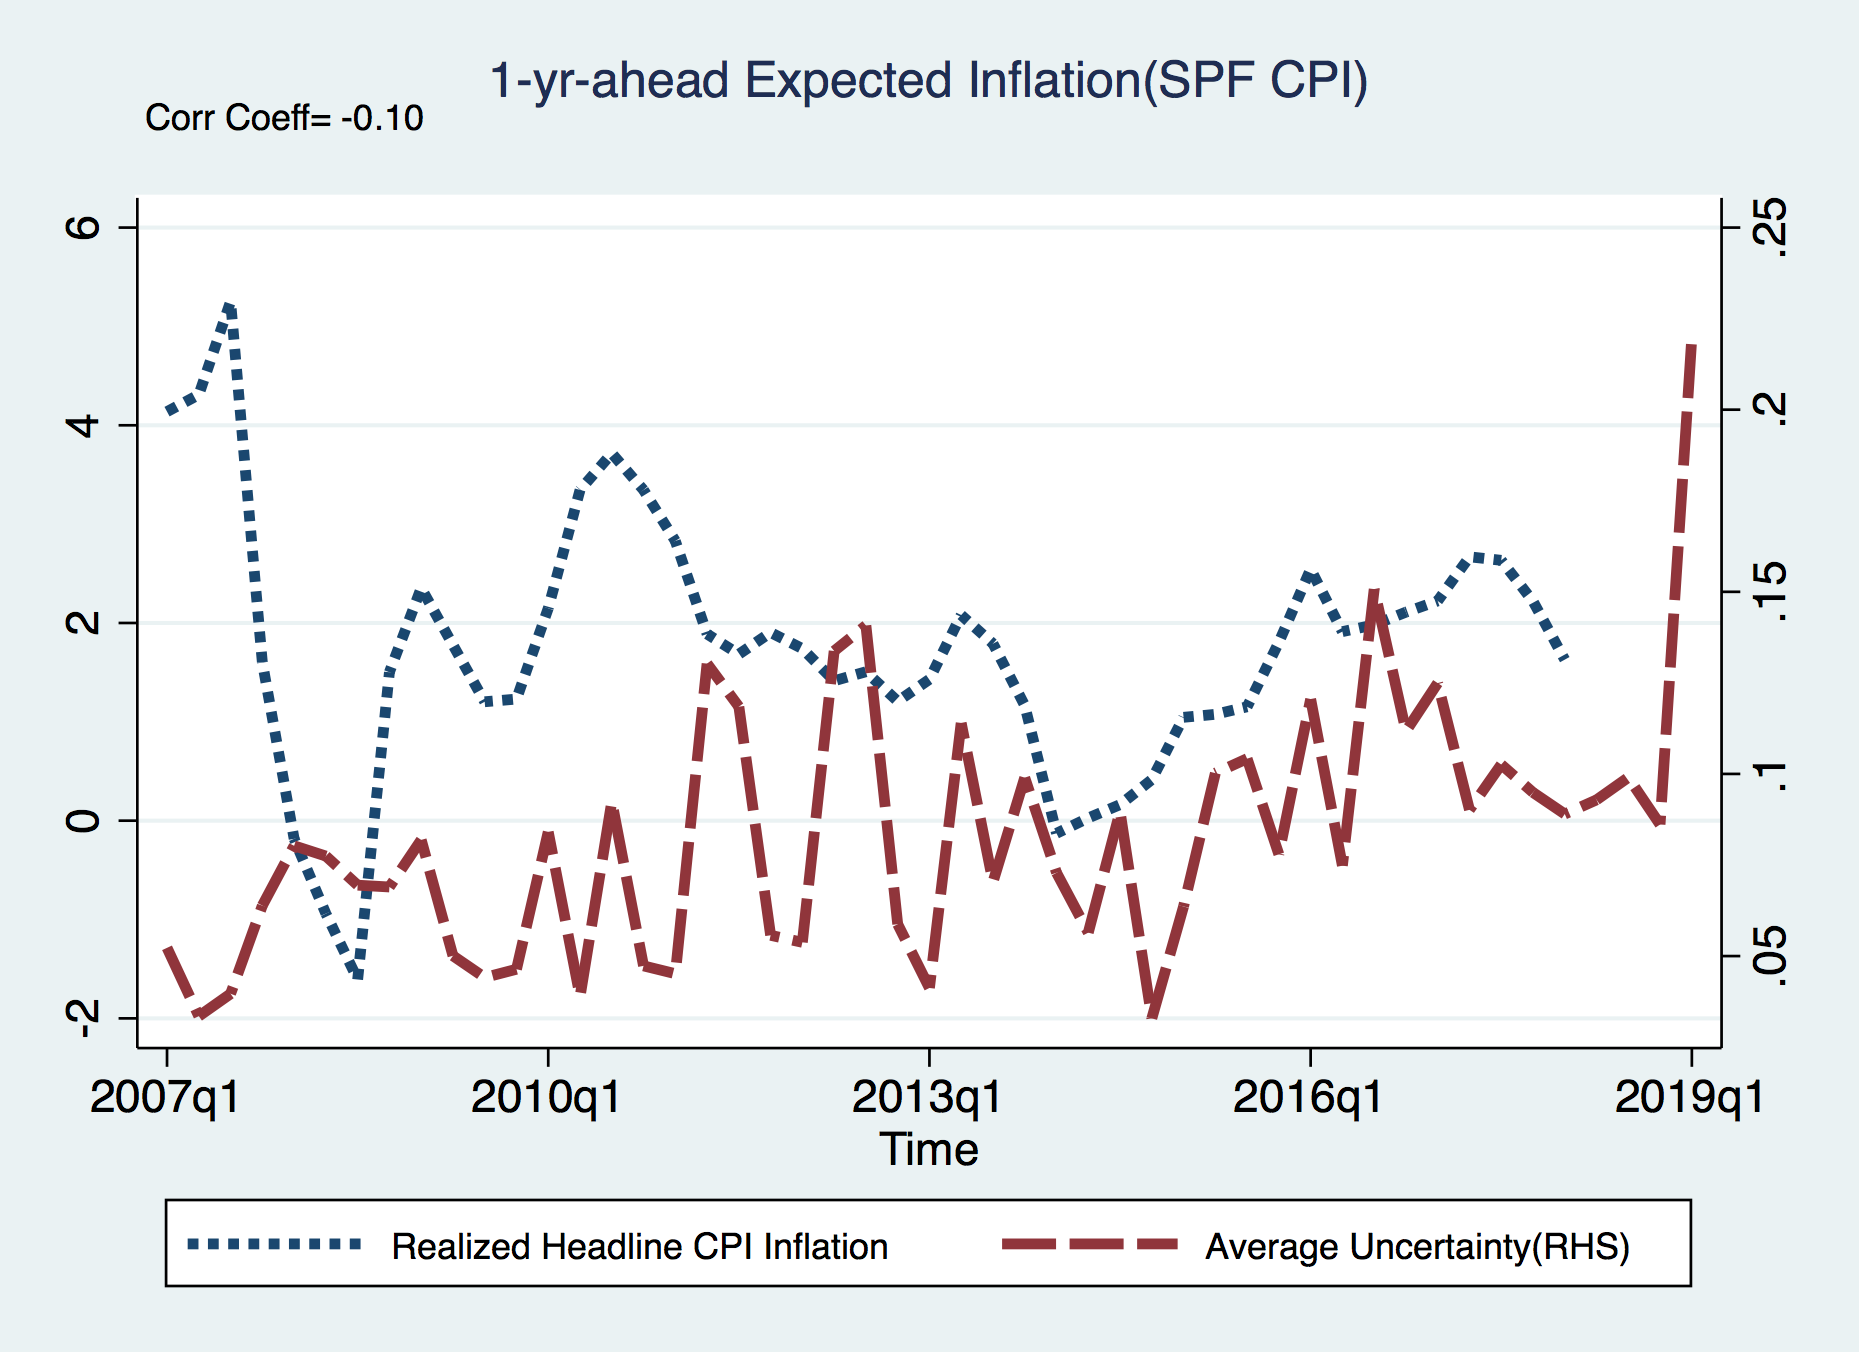
\includegraphics[width=0.3\textwidth]{figuresDraft/Inf1yf_CPIAU_varSPFCPIQ.png}
		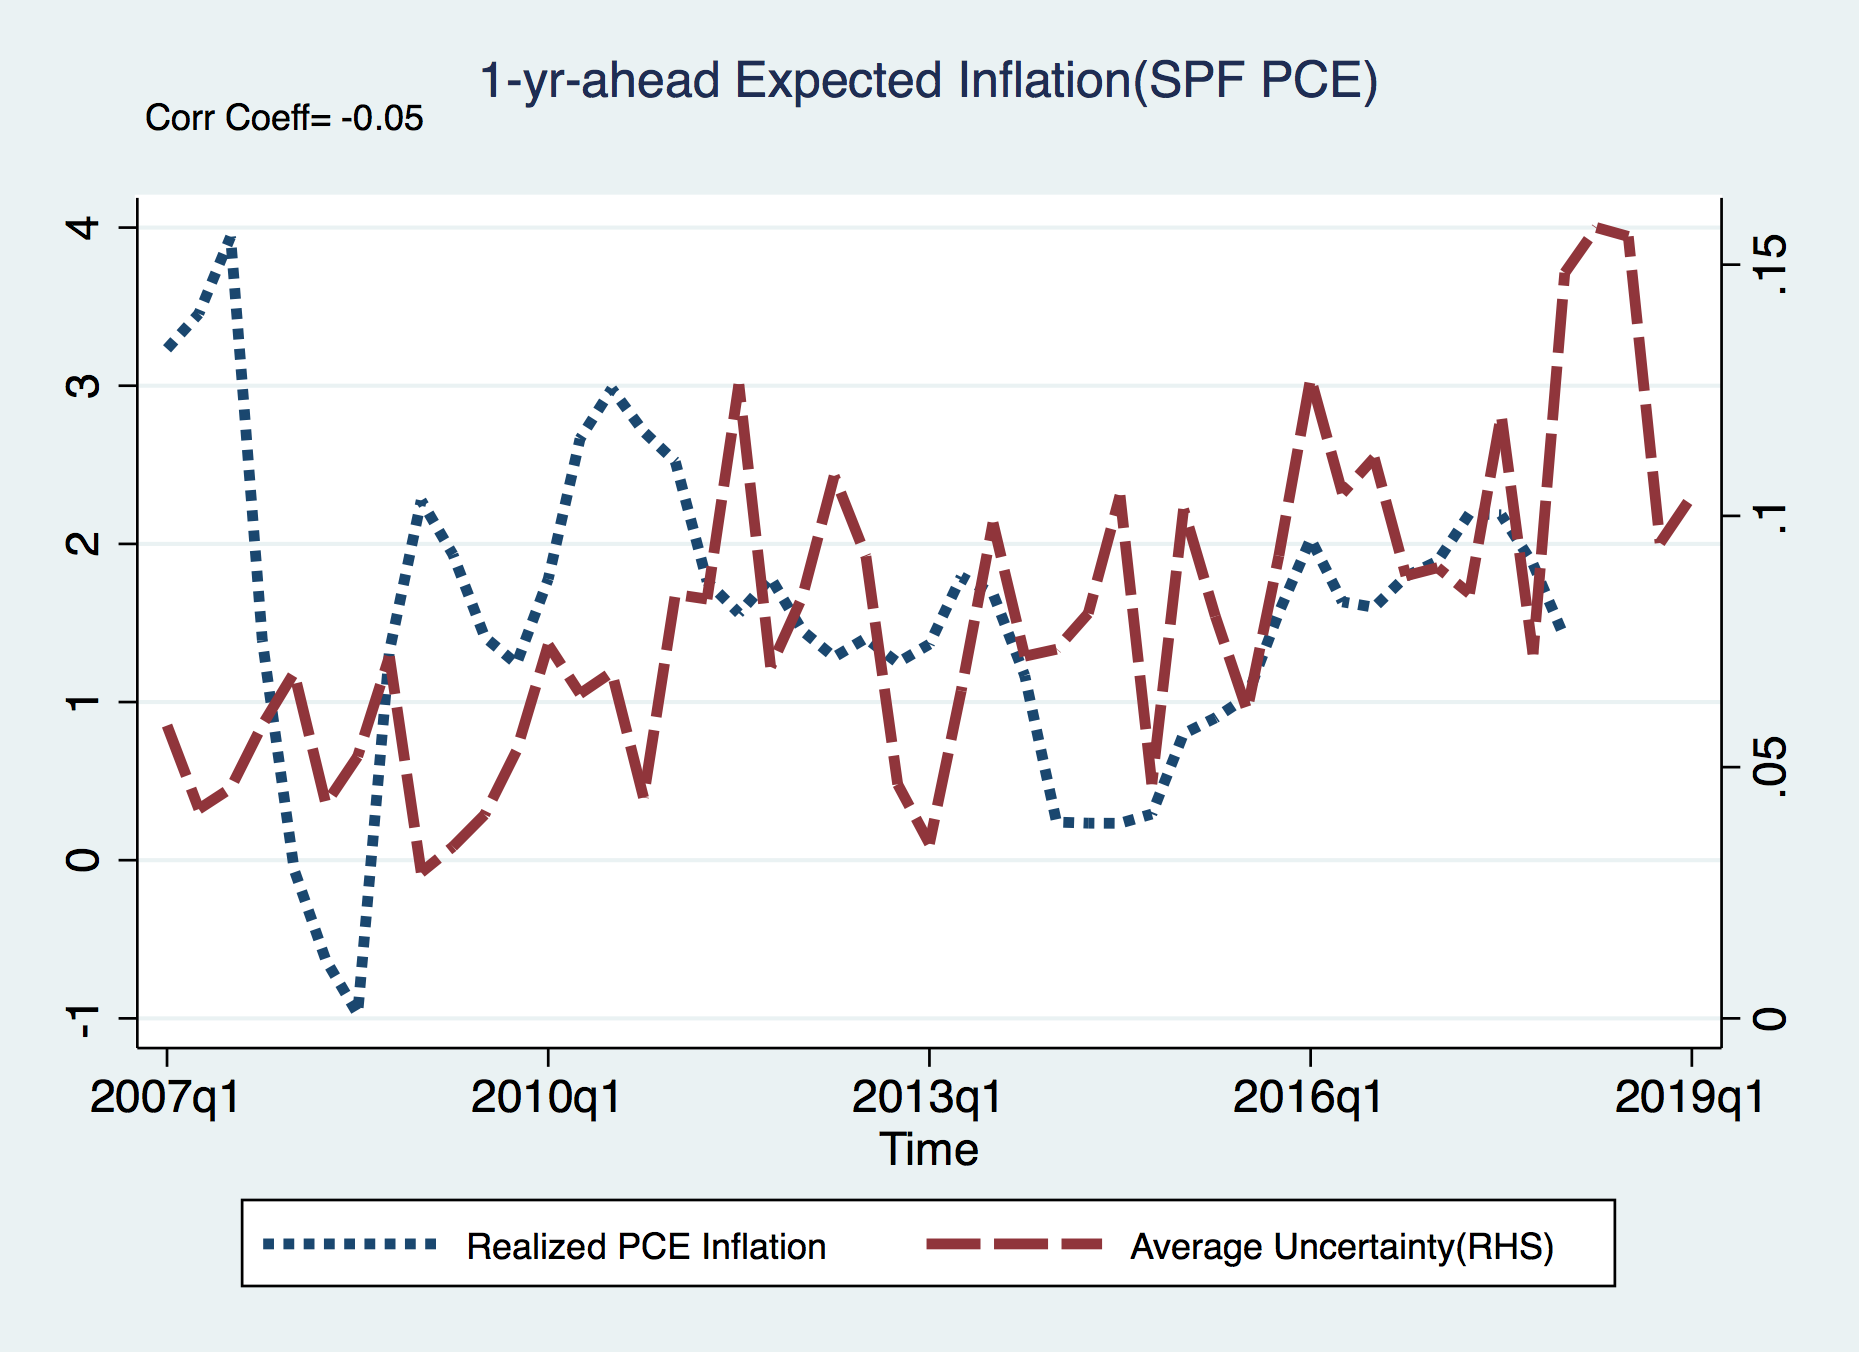
\includegraphics[width=0.3\textwidth]{figuresDraft/Inf1yf_PCE_varSPFPCEQ.png}
		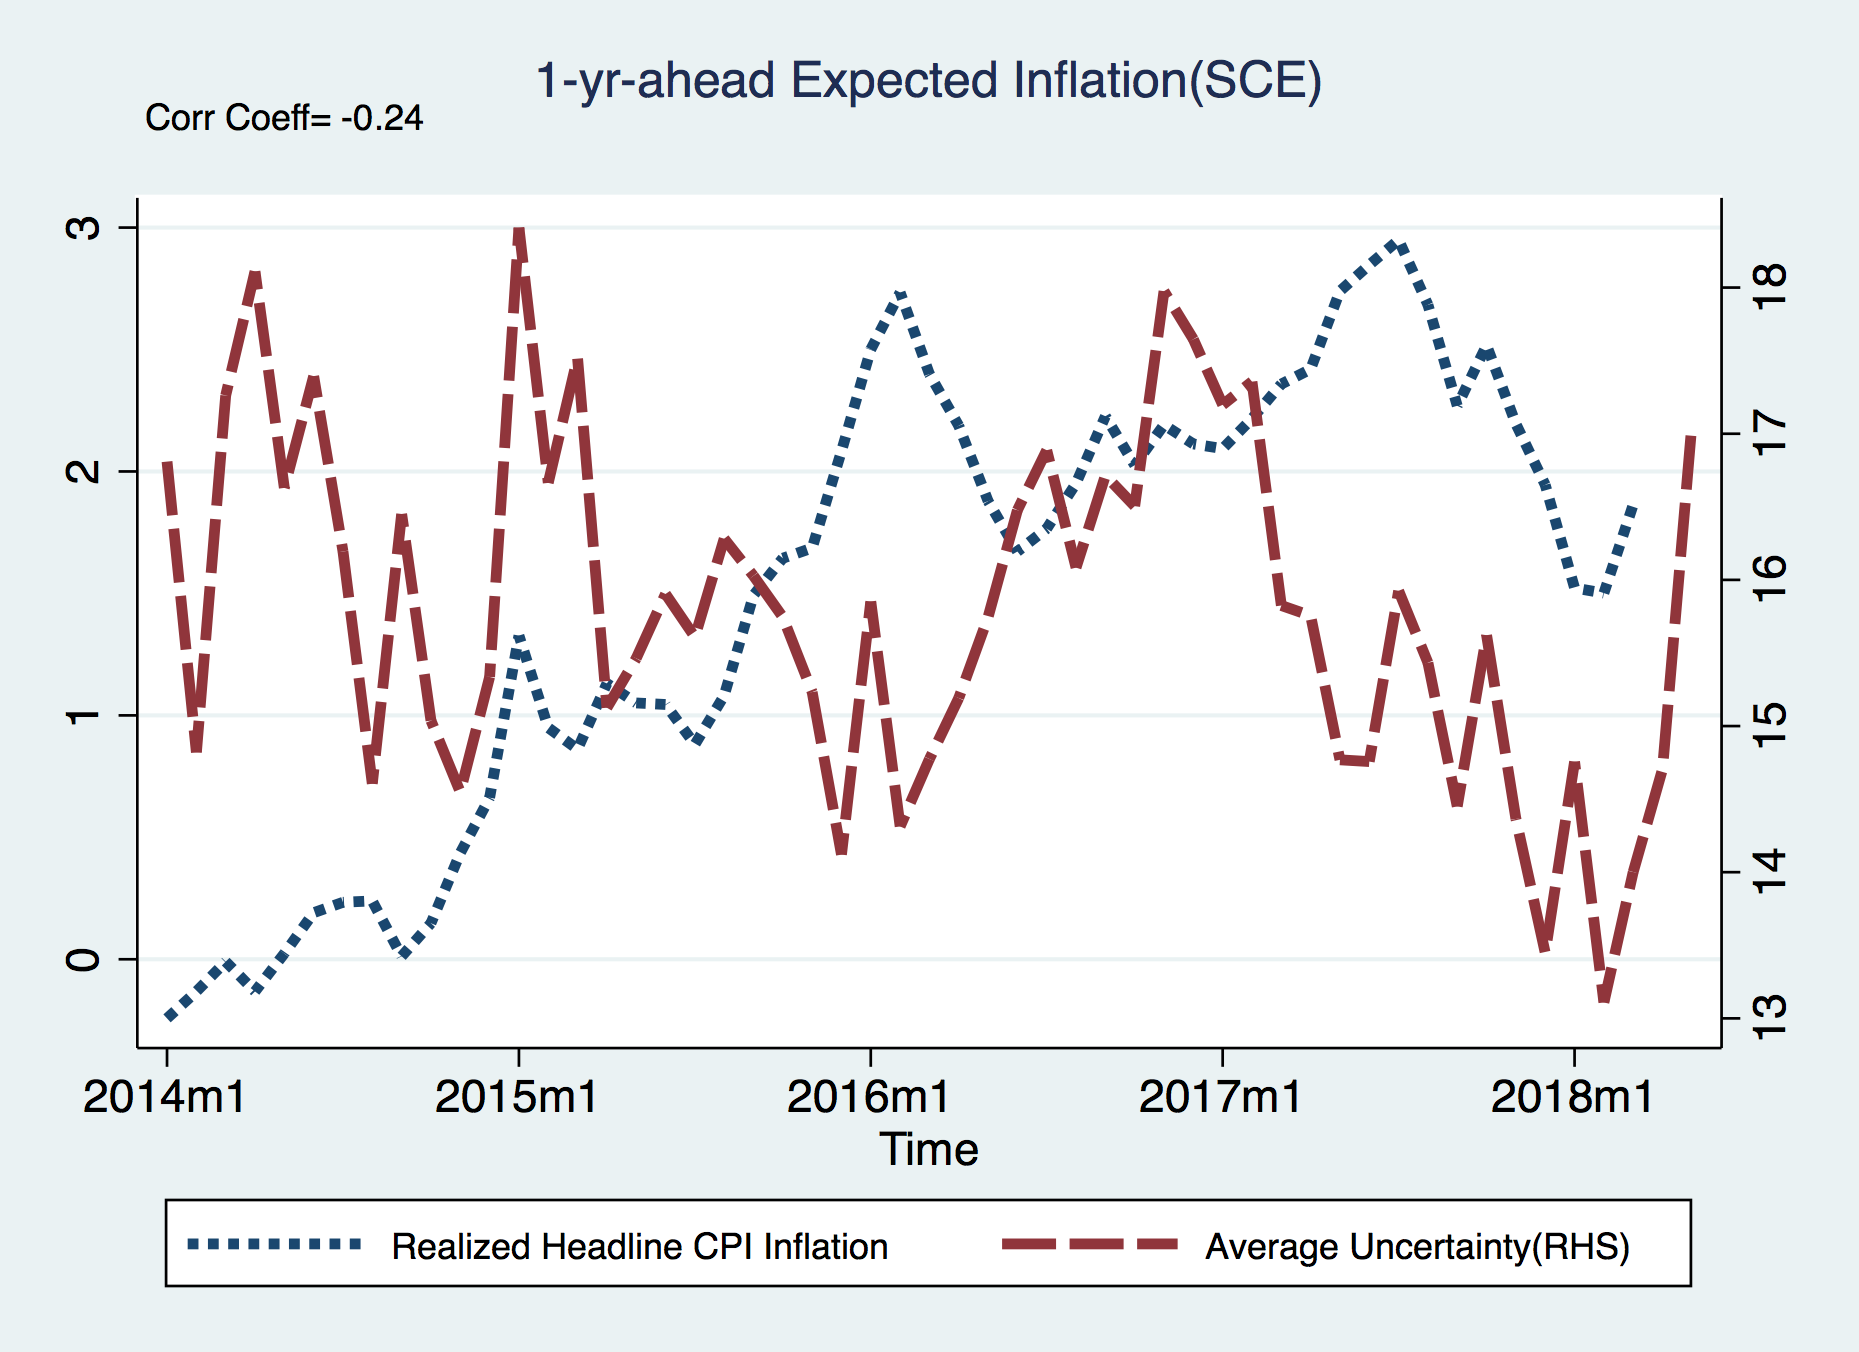
\includegraphics[width=0.3\textwidth]{figuresDraft/Inf1yf_CPIAU_varSCEM.png}
	\end{figure}

\end{frame}


\begin{frame}{Basic patterns: uncertainty and the size of forecast errors}
	\begin{figure}
		\centering
		\label{FEVar}
		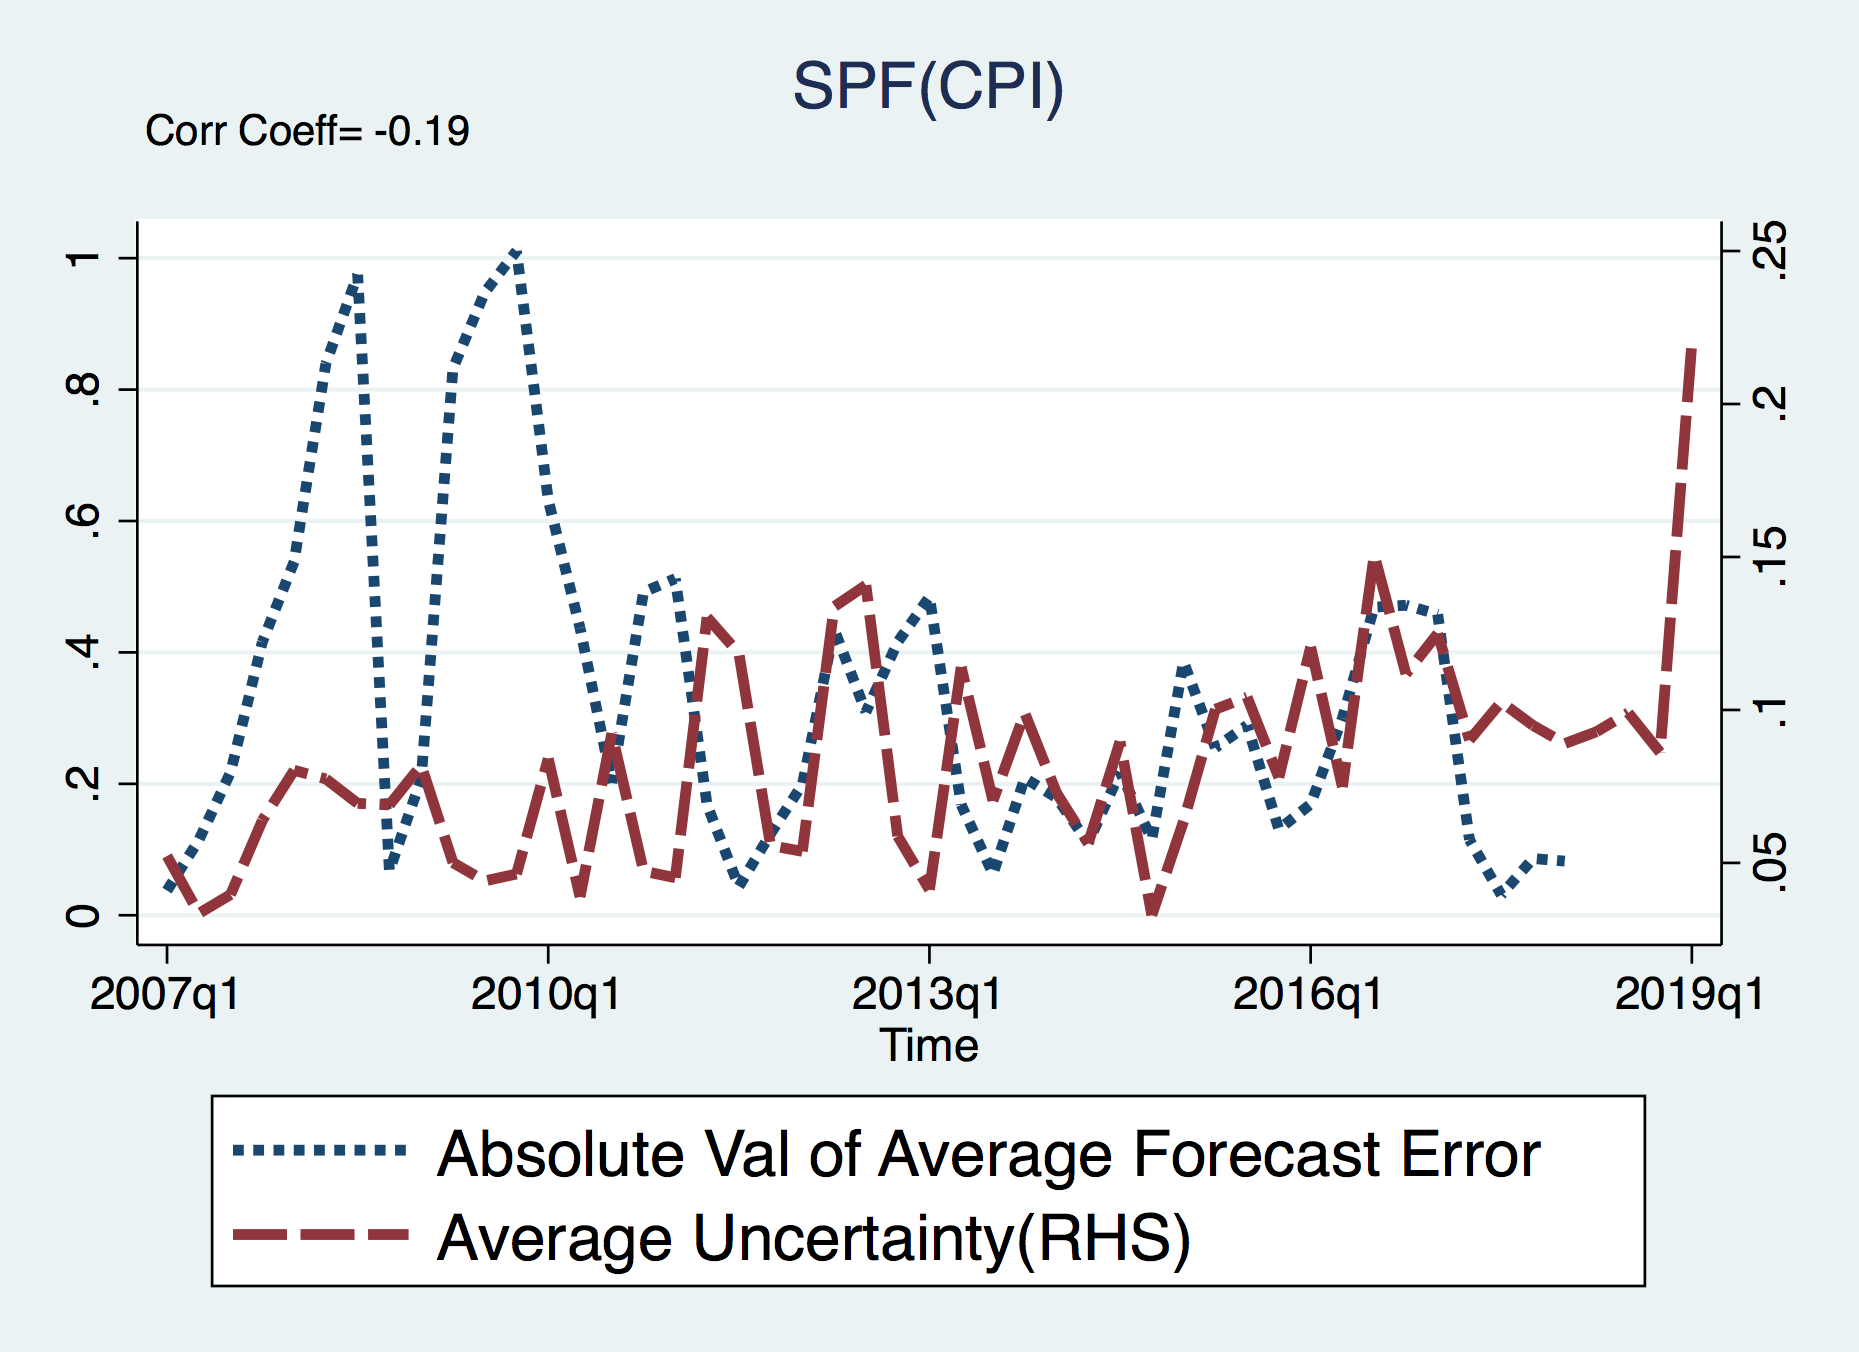
\includegraphics[width=0.3\textwidth]{figuresDraft/SPFCPI_abFE_varSPFCPIQ.png}
		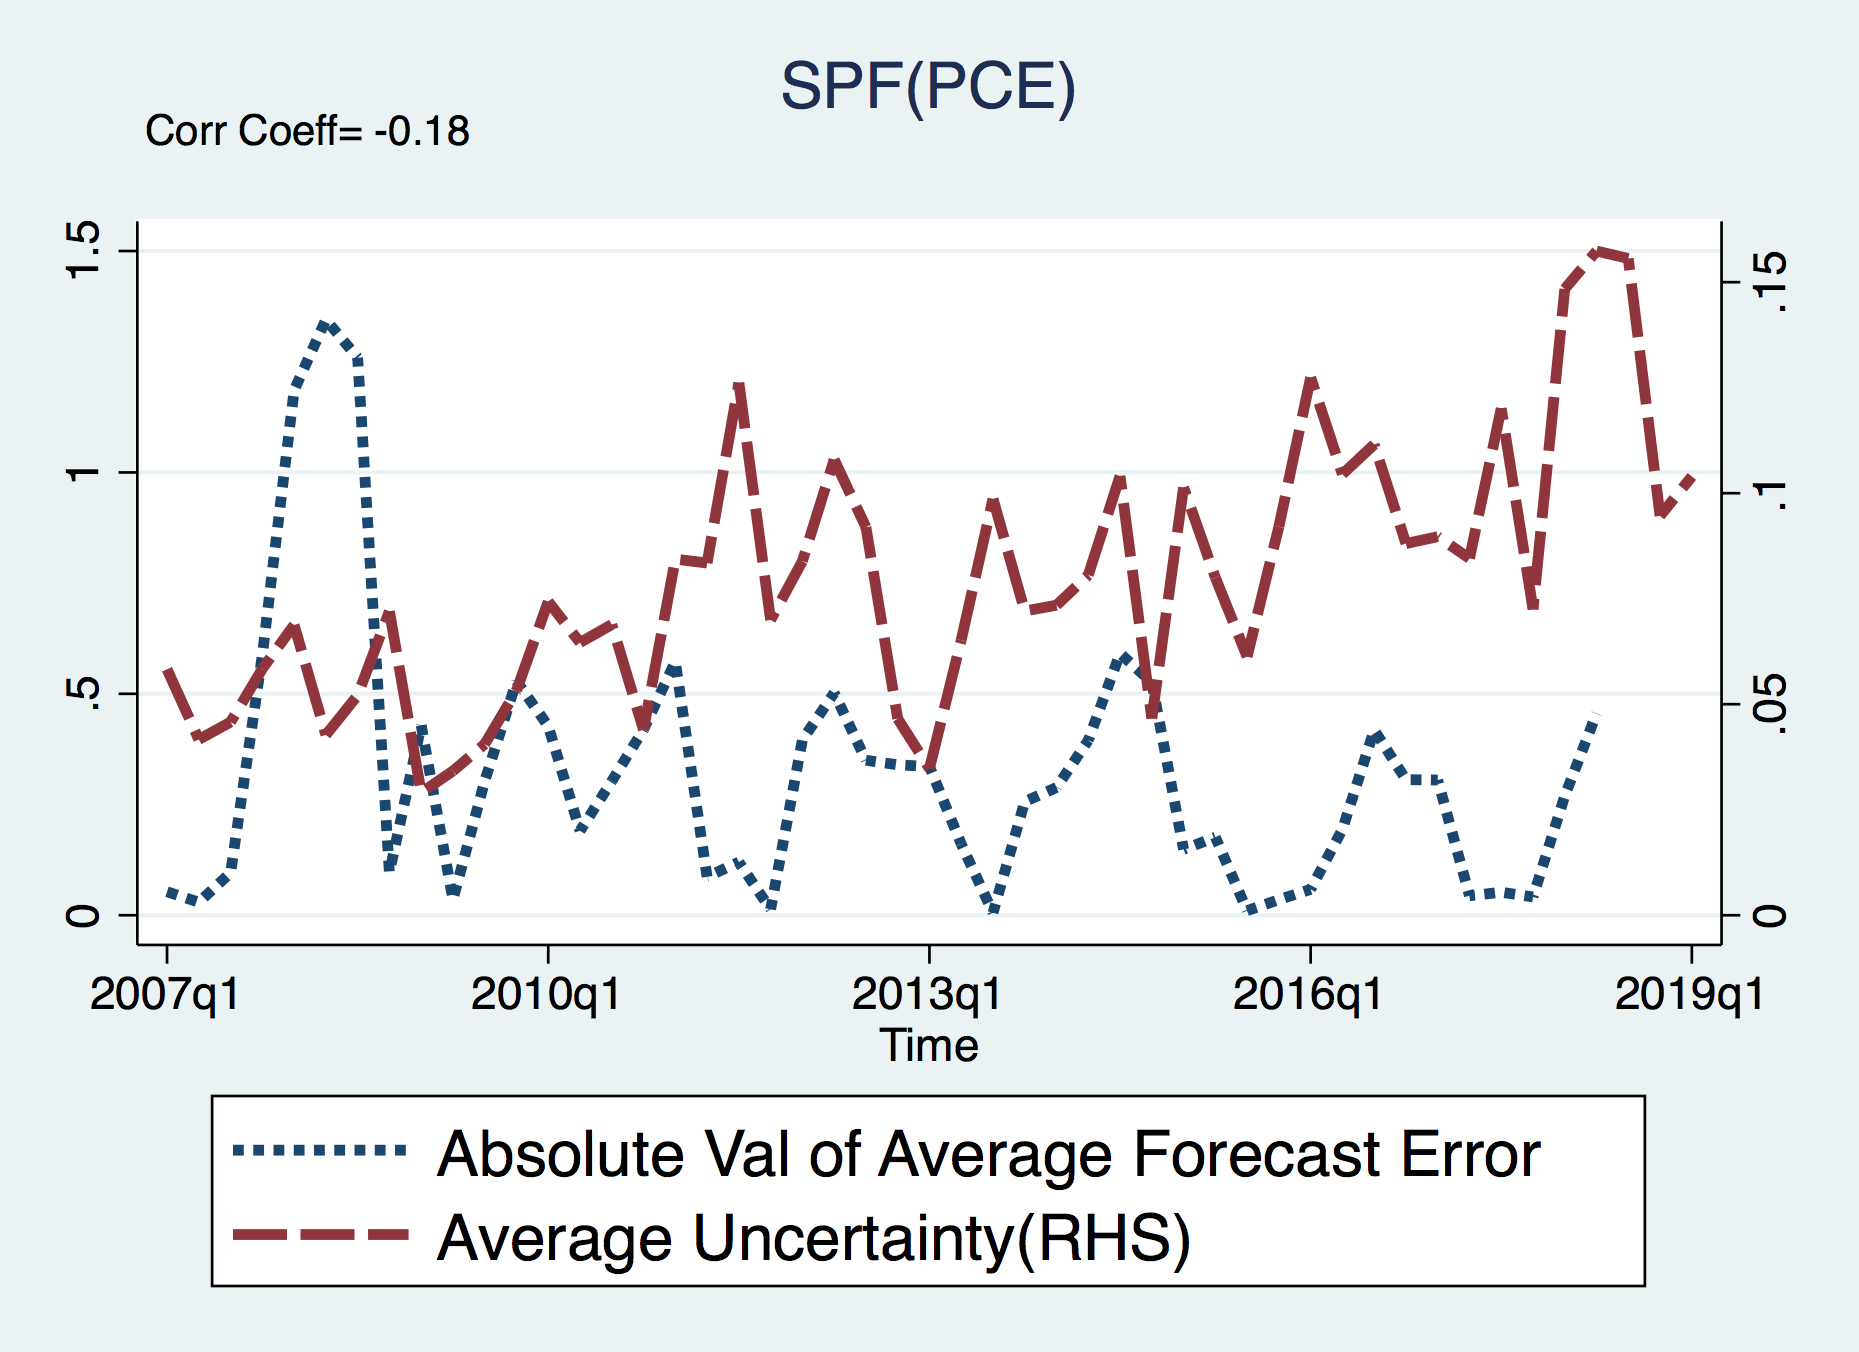
\includegraphics[width=0.3\textwidth]{figuresDraft/SPFPCE_abFE_varSPFPCEQ.png}
		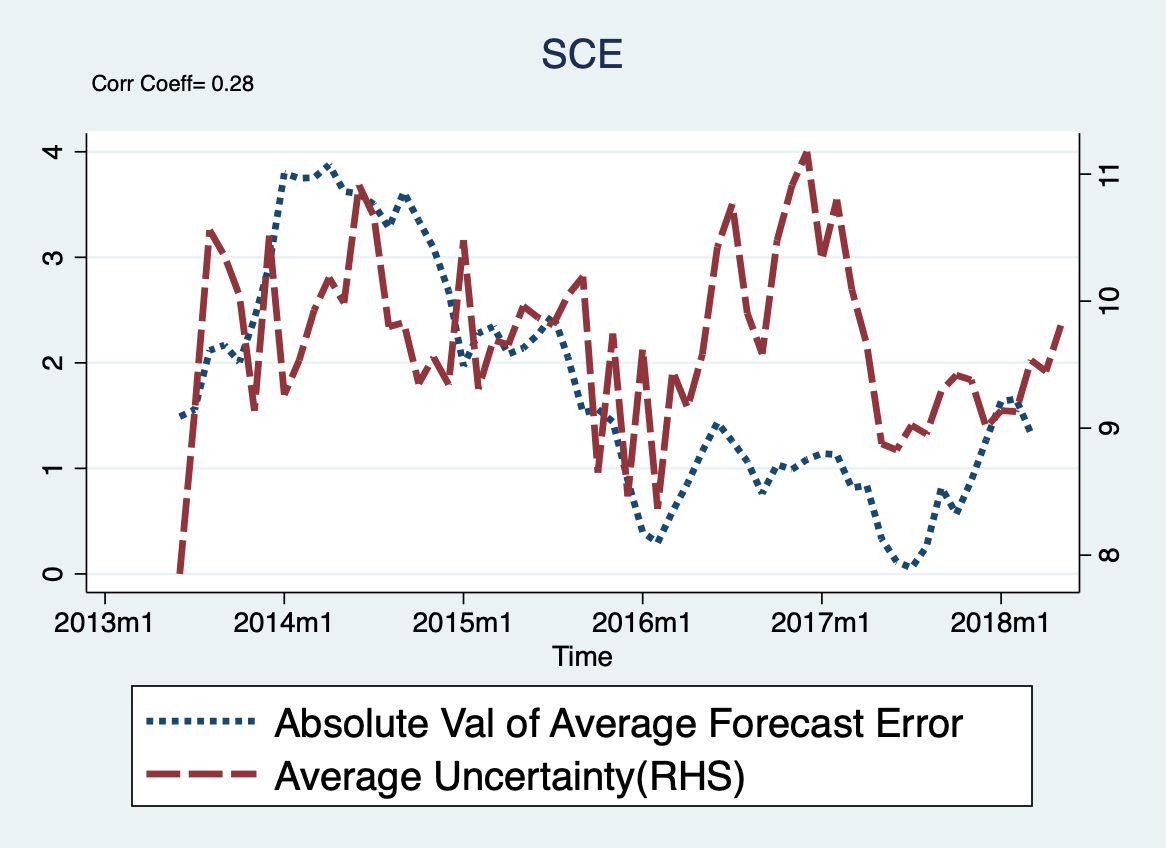
\includegraphics[width=0.3\textwidth]{figuresDraft/SCE_abFE_varSCEM.png}
	\end{figure}
\begin{itemize}
\item no evidence for positive correlation betwen high ex ante uncertainty and ex post forecast errors.
\end{itemize}
\end{frame}

\begin{frame}{Basic patterns: uncertainty and disagreement}
	\begin{figure}
		\centering
		\label{DisgVar}
		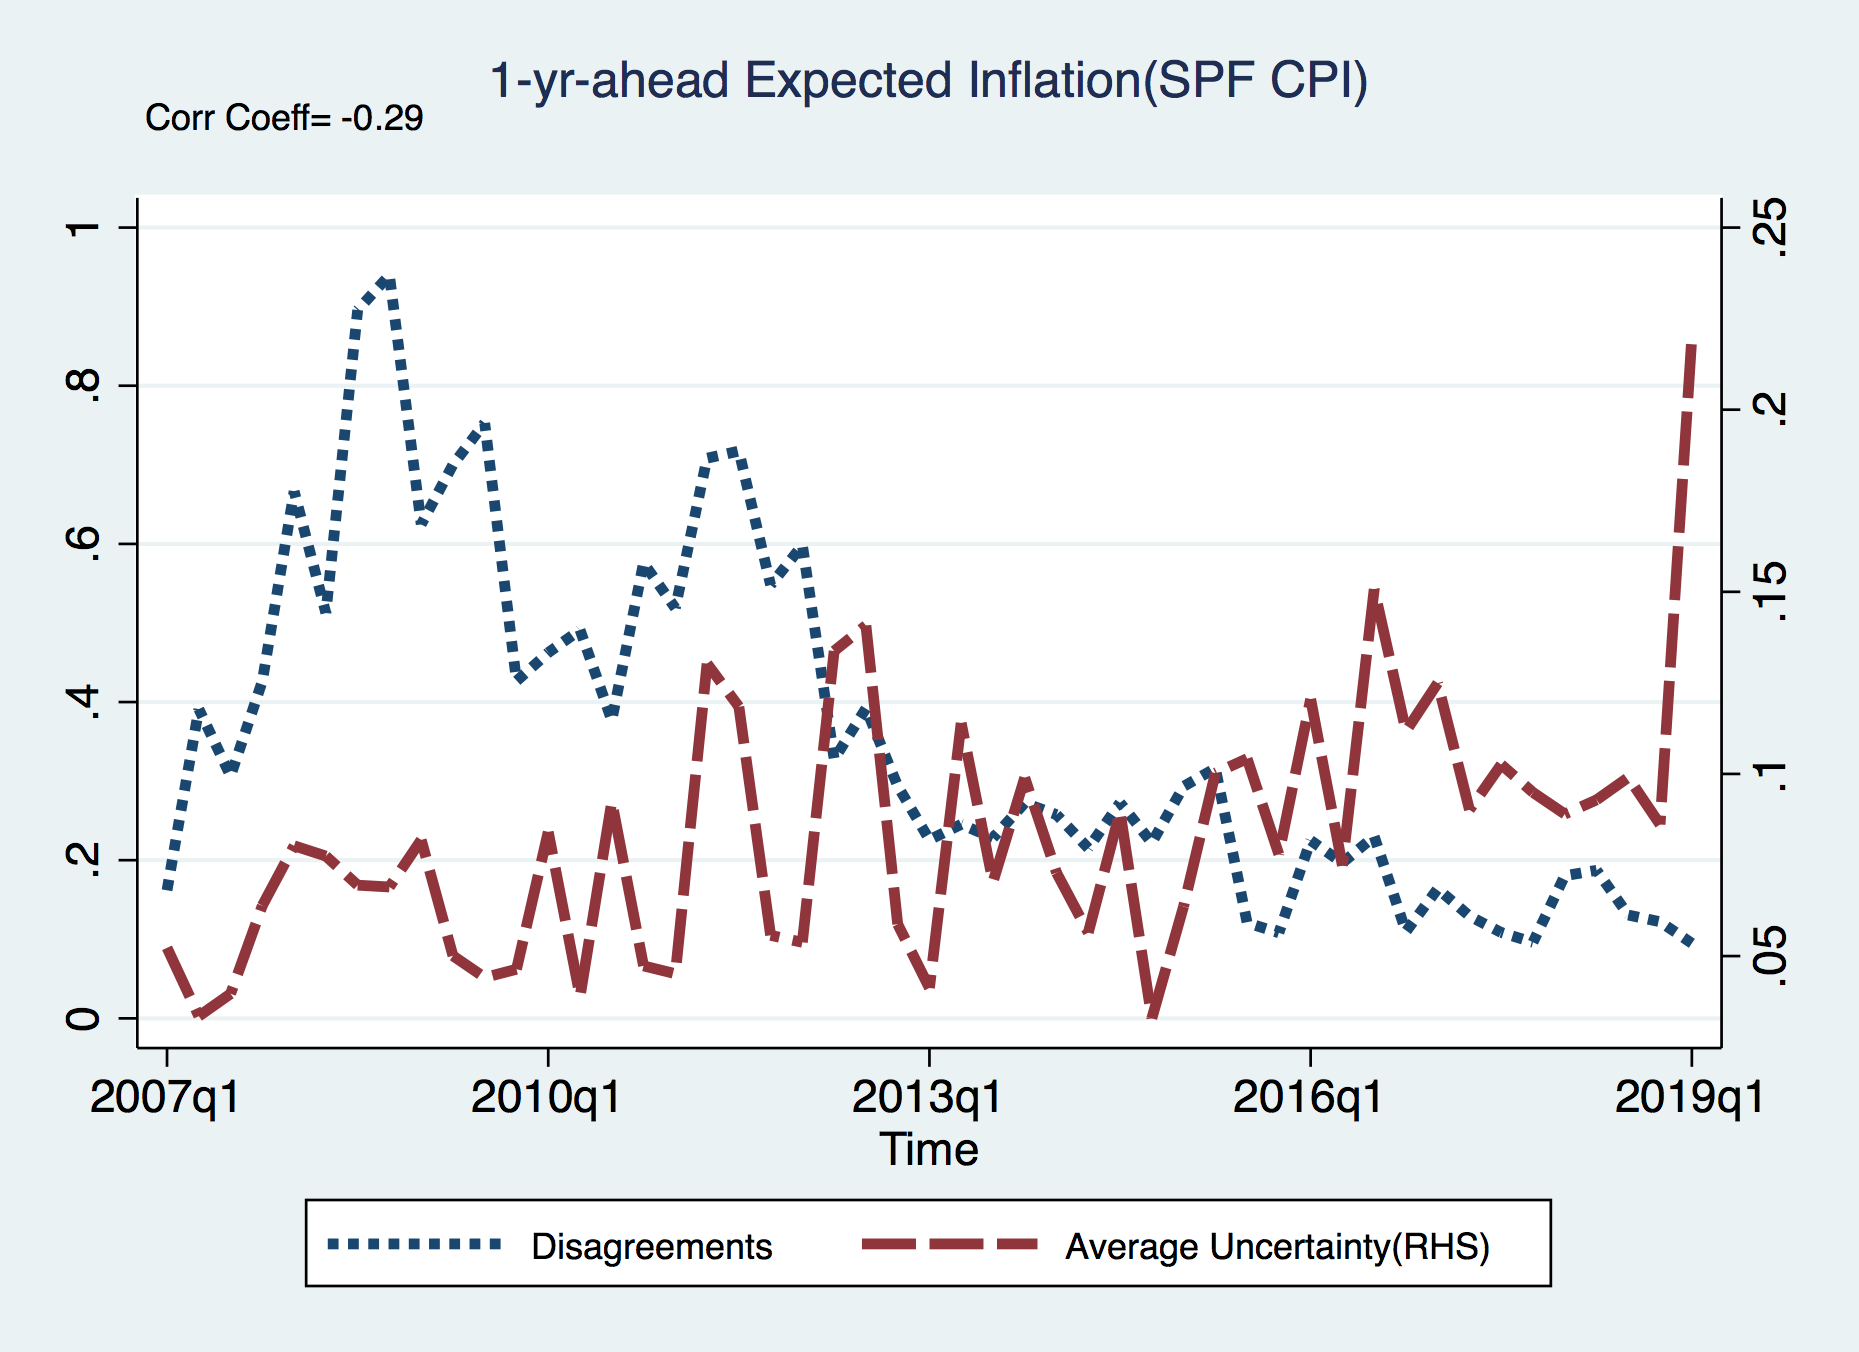
\includegraphics[width=0.3\textwidth]{figuresDraft/CPI_disg_varSPFCPIQ.png}
		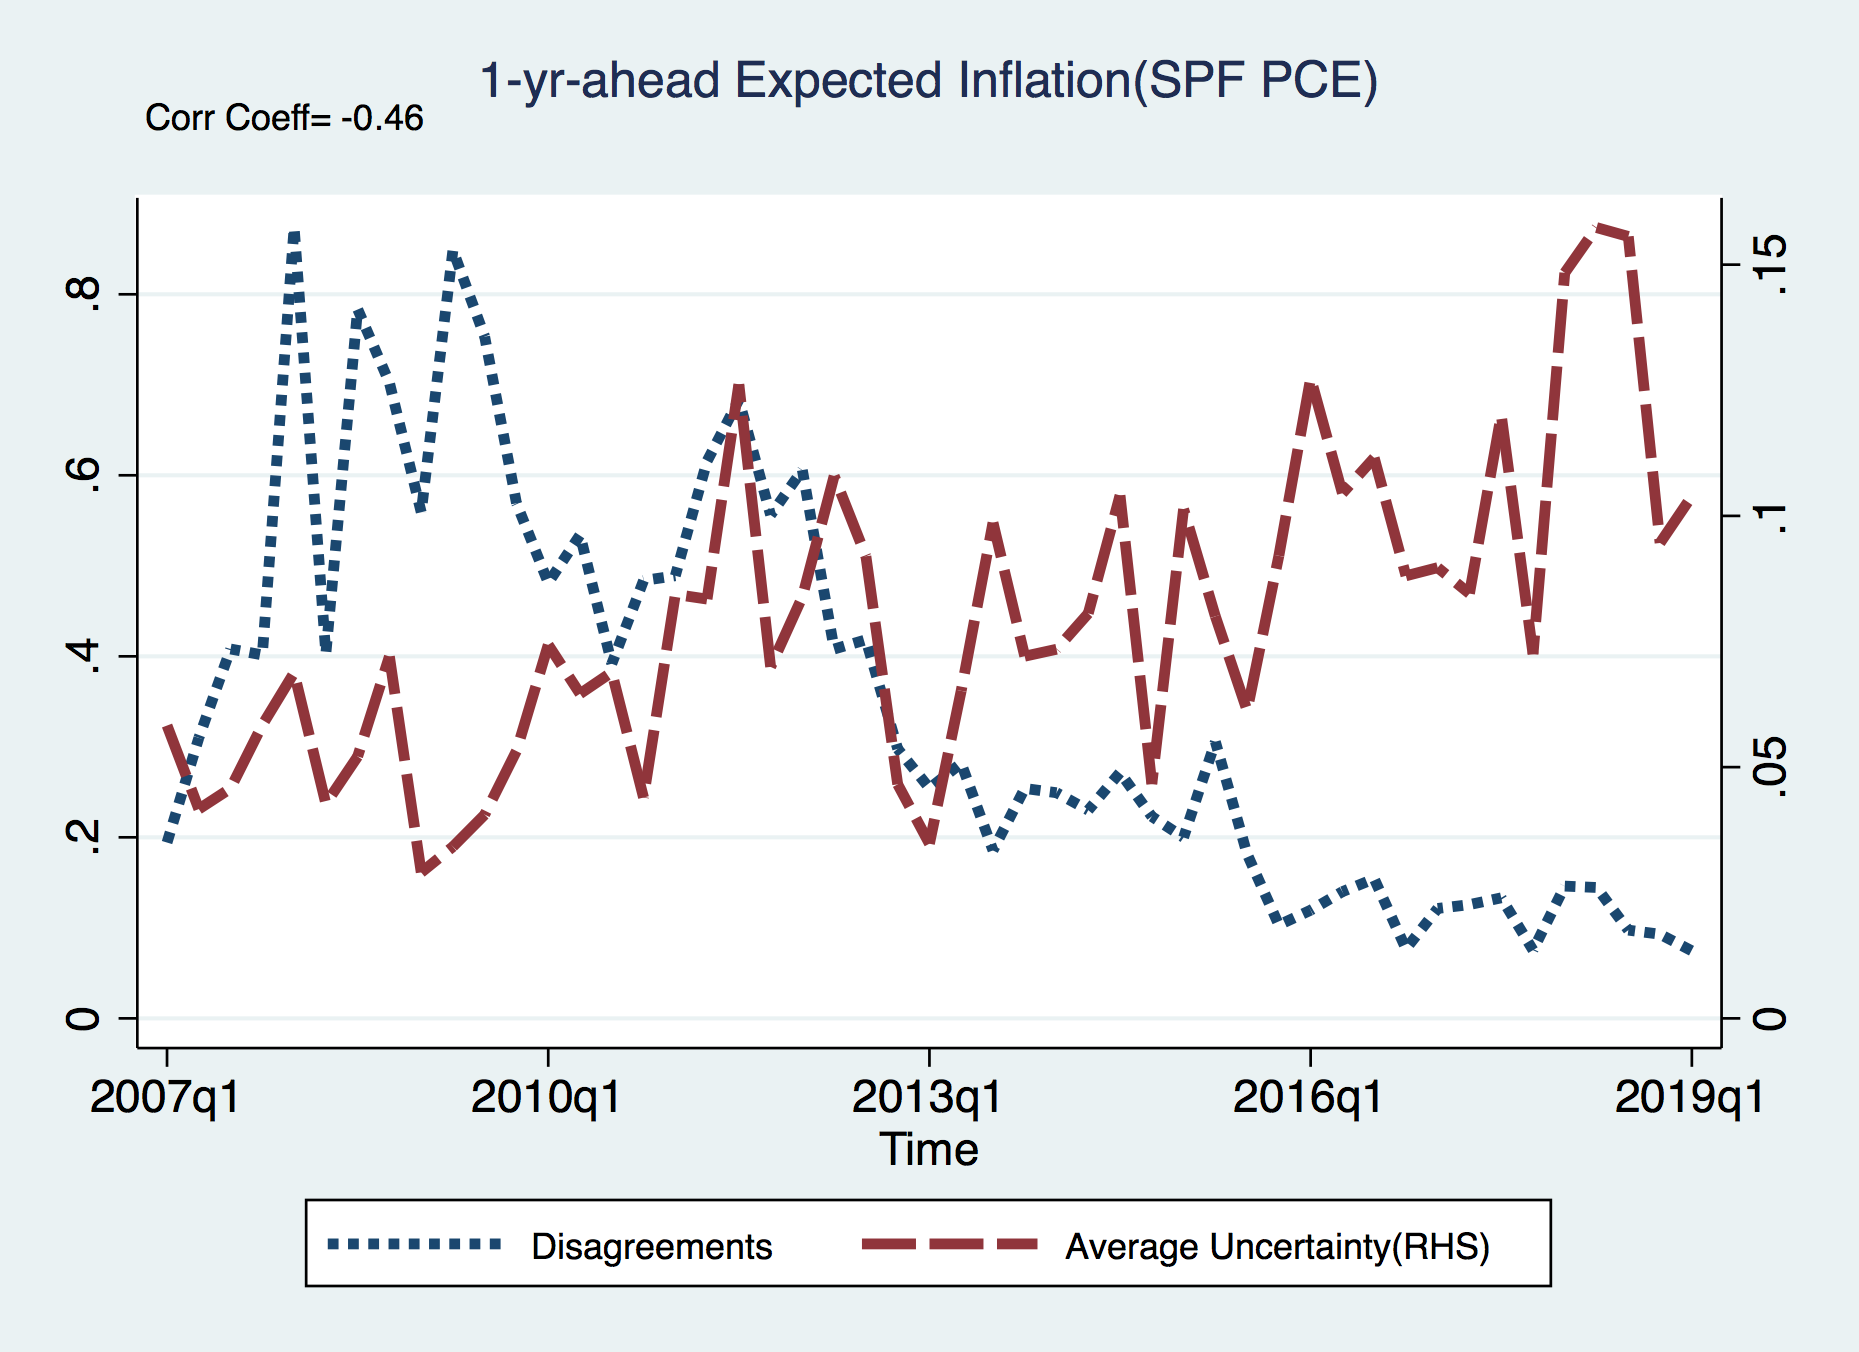
\includegraphics[width=0.3\textwidth]{figuresDraft/PCE_disg_varSPFPCEQ.png}
		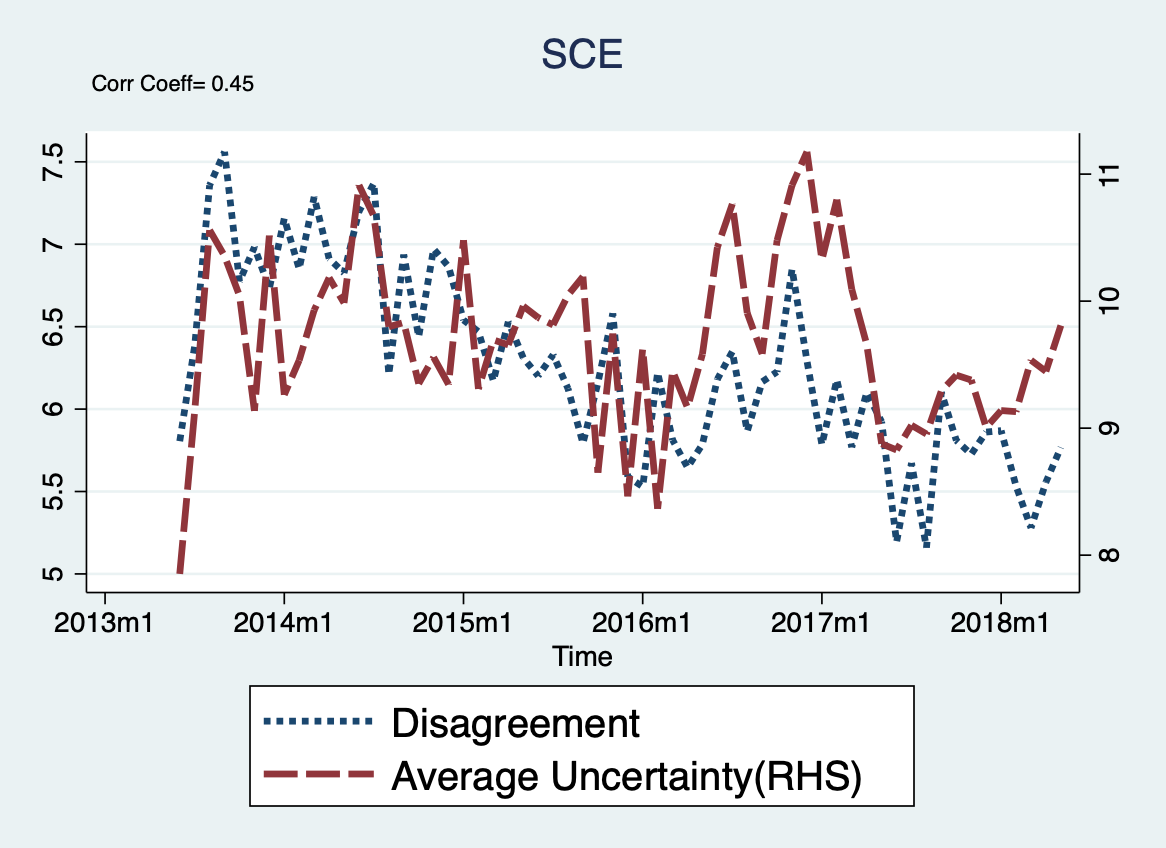
\includegraphics[width=0.3\textwidth]{figuresDraft/Q9_disg_varSCEM.png}
	\end{figure}
\begin{itemize}
	\item uncertainty are not the same as disagreement for professionals 
\end{itemize}
\end{frame}

\begin{frame}{Basic patterns: summary}
	\begin{itemize}
		\item uncertainty varies across time 
		\item uncertainty contains different information from widely  proxies such as disagreement and forecast error
	\end{itemize}
\end{frame}

\section{Theory}

\begin{frame}{AR(1) model of inflation}
	

\begin{itemize}
	
\item 	\textbf{Inflation process}	
	$$y_{t} = \rho y_{t-1} + \omega_t  $$ 
	$$\omega_t \sim N(0,\sigma^2_{\omega})$$

\item \textbf{Uncertainty}
		\begin{itemize}
			\item FIRE: time-invariant 
			\begin{eqnarray*}\label{VarREPop}
				\overline{Var}^*_{t+h|t} = \sum^{h}_{s=1}\rho^{2s} \sigma^2_{\omega}
			\end{eqnarray*}
			
			\item SE: time-invariant 
			\begin{eqnarray*}\label{VarSEPopRE}
				\overline{Var}^{se}_{t+h|t} = \sum^{+\infty}_{\tau =0} \lambda (1-\lambda)^\tau \overline{Var}^*_{t+h|t-\tau}
			\end{eqnarray*}
			
			\item NI: time-variant but quantitatively tiny due to highly efficient Kalman gain
			
			\begin{eqnarray*}\label{VarNIPopRE}
				\overline{Var}^{ni}_{t+h|t} = \rho^{2h} \overline{Var}^{ni}_{t|t} + \overline{Var}^*_{t+h|t}
			\end{eqnarray*}
		\end{itemize}
		
	\end{itemize}
	
\end{frame}

\begin{frame}{Stocastic volatility (UCSV) inflation process (\citet{stock2007has})}

\begin{itemize}
\item \textbf{Inflation process}
\begin{eqnarray*}
\begin{split}
& y_t = \theta_t + \eta_t,\quad \textrm{where } \eta_t =\sigma_{\eta,t} \xi_{\eta,t} \\
& \theta_t = \theta_{t-1} + \epsilon_t, \quad \textrm{where }  \epsilon_t =\sigma_{\epsilon,t} \xi_{\epsilon,t} \\
& \log\sigma^2_{\eta,t} = \log\sigma^2_{\eta,t-1} + \mu_{\eta,t} \\
& \log\sigma^2_{\epsilon,t} = \log\sigma^2_{\epsilon,t-1} + \mu_{\epsilon,t} 
\end{split}
\end{eqnarray*}

\begin{eqnarray*}
\begin{split}
& \xi_t =[\xi_{\eta,t},\xi_{\epsilon,t}] \sim N(0,I_2) \\
& \mu_{t} = [\mu_{\eta,t},\mu_{\epsilon,t}]' \sim N(0,\gamma I_2) 
\end{split}
\end{eqnarray*}
\end{itemize}

\end{frame}


\begin{frame}{UCSV inflation process}
	
	\begin{itemize}
		\item \textbf{Uncertainty}
		\begin{itemize}
			\item FIRE: time-varying  \begin{eqnarray*}\label{VARRESVPop}
			\begin{split}
			\overline{Var}^*_{t+h|t} = \sum_{k=1}^h exp^{- 0.5k\gamma_{\eta}} \sigma^2_{\eta,t}  +  exp^{- 0.5 h \gamma_{\epsilon}} \sigma^2_{\epsilon,t} 
			\end{split} 
			\end{eqnarray*}
			
			\item SE: time-varying 
			\begin{eqnarray*}
		\overline {Var}^{se}_{t+h|t} = \sum^{\infty}_{\tau=0} (1-\lambda)^\tau\lambda\overline{Var}^*_{t+h|t-\tau} 
			\end{eqnarray*}
			
			\item NI (1-step-ahead): time-varying 
		\begin{eqnarray*}
		\overline{Var}^\theta_{t|t-1} = \overline{Var}^\theta_{t-1|t-1} + Var^*_{t|t-1}(y_t) 
		\end{eqnarray*}
			
		\end{itemize}
	\end{itemize}
	
\end{frame}


\section{Estimation}
\begin{frame}{Minimum distance estimation}
	
	\begin{eqnarray*}
	\widehat \Omega = \underset{\{\Omega \in \Gamma\} }{argmin} (M_{\textrm{data} } - F^{o}(\Omega, Y)) W  (M_{\textrm{data} } - F^{o}(\Omega, Y))'
	\end{eqnarray*}
	
	\begin{itemize}
		\item  $\Omega$: parameters of the particular $o \in \{{fire}, {se}, {ni} \} \times \{ar, sv\}$
		\item  $\Gamma$: constraints for the parameter. 
		\item $M_{data}$: data moments
		\item $F$ model moments according to a particular theory $o$, a function of parameters $\Omega$ as well as the $Y$, the real-time data (including history) up to each point of the time $t$
		\item  $W$: weight matrix, identity matrix for now 
	\end{itemize}
		
\end{frame}

\subsection{AR(1)}

\begin{frame}{Results: professionals and SEAR}
	\begin{figure}[ht]
		\label{SE_diag_SPF}
		\begin{subfigure}[b]{0.19\textwidth}
			\centering
			\caption{forecast}
			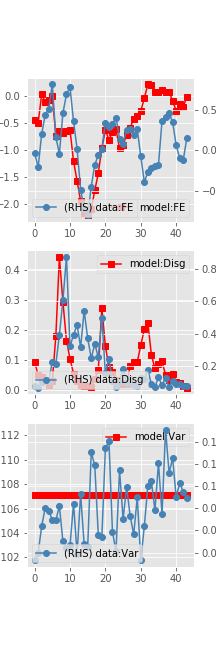
\includegraphics[width=\textwidth, height = 0.8\textheight]{figuresDraft/spf_se_est_diag0.png}
		\end{subfigure}
		\hfill
		\begin{subfigure}[b]{0.19\textwidth}
			\caption{FE}
			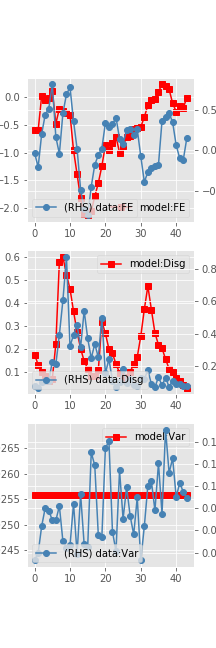
\includegraphics[width=\textwidth, height = 0.8\textheight]{figuresDraft/spf_se_est_diag1.png}
		\end{subfigure}
		\hfill
		\begin{subfigure}[b]{0.19\textwidth}
			\caption{forecast/FE}
			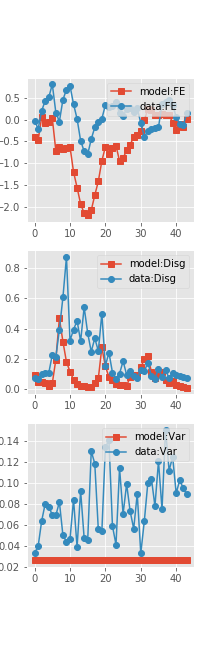
\includegraphics[width=\textwidth, height = 0.8\textheight]{figuresDraft/spf_se_est_diag2.png}
		\end{subfigure}
		\hfill
		\begin{subfigure}[b]{0.19\textwidth}
			\caption{FE/var}
			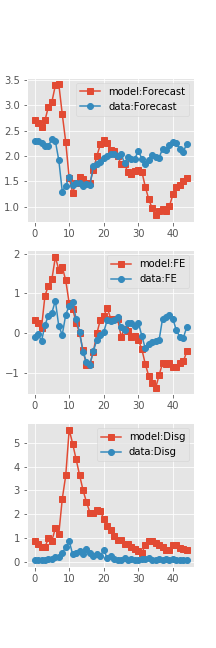
\includegraphics[width=\textwidth, height = 0.8\textheight]{figuresDraft/spf_se_est_diag3.png}
		\end{subfigure}
		\hfill
		\begin{subfigure}[b]{0.19\textwidth}
			\caption{FE/var/Disg}
			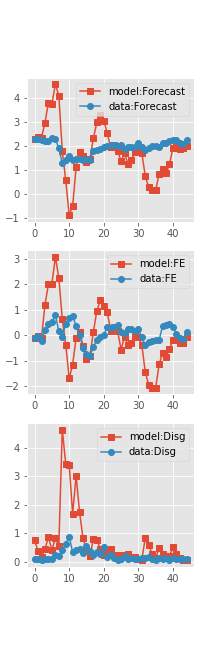
\includegraphics[width=\textwidth, height = 0.8\textheight]{figuresDraft/spf_se_est_diag4.png}
		\end{subfigure}
	\end{figure}
\end{frame}


\begin{frame}{Results: households and SEAR}
	\begin{figure}[ht]
	\label{SE_diag_SCE}
	\begin{subfigure}[b]{0.19\textwidth}
		\centering
		\caption{forecast}
			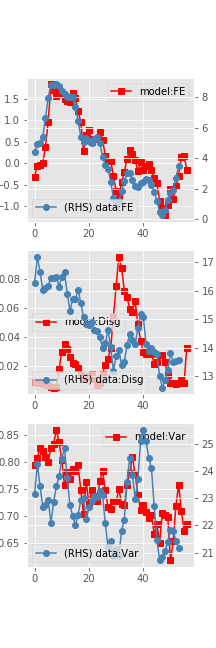
\includegraphics[width=\textwidth, height = 0.8\textheight]{figuresDraft/sce_se_est_diag0.png}
	\end{subfigure}
	\hfill
	\begin{subfigure}[b]{0.19\textwidth}
		\caption{FE}
			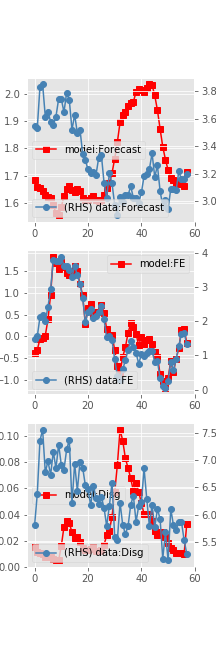
\includegraphics[width=\textwidth, height = 0.8\textheight]{figuresDraft/sce_se_est_diag1.png}
	\end{subfigure}
\hfill
\begin{subfigure}[b]{0.19\textwidth}
	\caption{forecast/FE}
	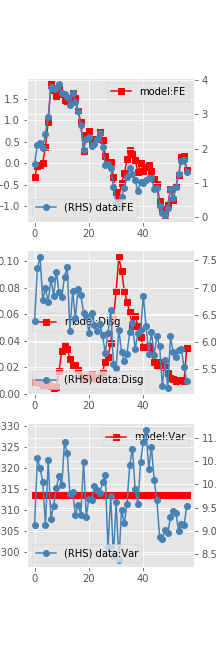
\includegraphics[width=\textwidth, height = 0.8\textheight]{figuresDraft/sce_se_est_diag2.png}
\end{subfigure}
\hfill
\begin{subfigure}[b]{0.19\textwidth}
	\caption{FE/var}
	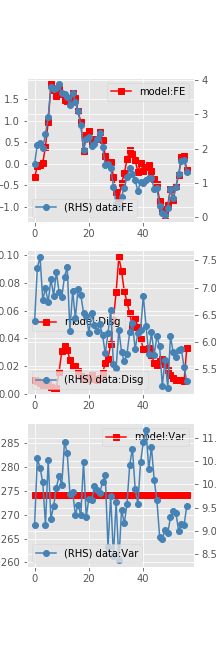
\includegraphics[width=\textwidth, height = 0.8\textheight]{figuresDraft/sce_se_est_diag3.png}
\end{subfigure}
\hfill
\begin{subfigure}[b]{0.19\textwidth}
	\caption{FE/var/Disg}
	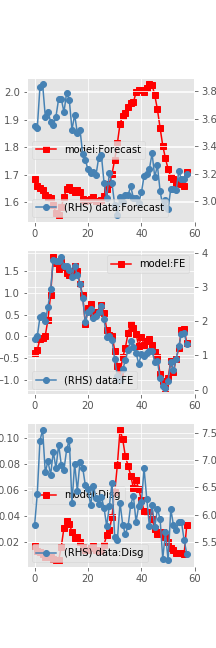
\includegraphics[width=\textwidth, height = 0.8\textheight]{figuresDraft/sce_se_est_diag4.png}
\end{subfigure}
\end{figure}
\end{frame}

\begin{frame}{SE parameter estimate}
	\begin{table}
		\centering
		\caption{Minimum Distance Estimates of Parameters of SE}
		\label{GMM_Est_SE_Table}
		\begin{tabular}{lllll}
			\hline 
			0        & 1    & 2   & SE: $\hat\lambda_{SPF}$(Q) & SE: $\hat\lambda_{SCE}$(M) \\
			\hline 
			Forecast &      &     & 0.04                       & 1                          \\
			FE       &      &     & 0.05                       & 0.19                       \\
			FE       & Disg &     & 0.17                       & 0.19                       \\
			FE       & Var  &     & 0.16                       & 0.18                       \\
			FE       & Disg & Var & 0.53                       & 0.18                      \\
			\hline 
		\end{tabular}
	\end{table}
\begin{itemize}
	\item $\lambda$: update rate in SE
\end{itemize}
\end{frame}


\begin{frame}{Results: professionals and NIAR}
	\begin{figure}[ht]
		\label{NI_diag_SPF}
		\begin{subfigure}[b]{0.19\textwidth}
			\centering
			\caption{forecast}
			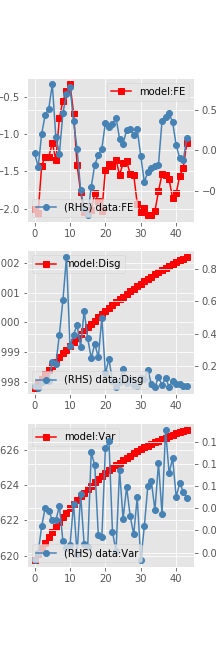
\includegraphics[width=\textwidth, height = 0.8\textheight]{figuresDraft/spf_ni_est_diag0.png}
		\end{subfigure}
		\hfill
		\begin{subfigure}[b]{0.19\textwidth}
			\caption{FE}
			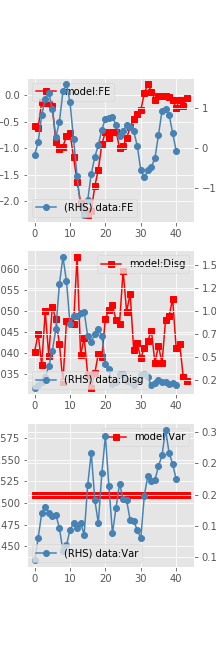
\includegraphics[width=\textwidth, height = 0.8\textheight]{figuresDraft/spf_ni_est_diag1.png}
		\end{subfigure}
		\hfill
		\begin{subfigure}[b]{0.19\textwidth}
			\caption{forecast/FE}
			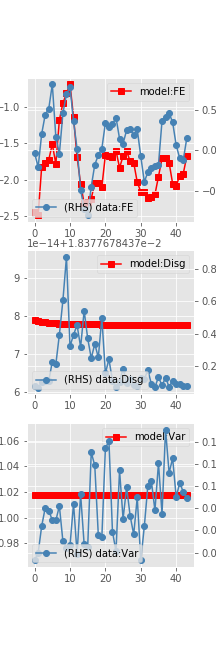
\includegraphics[width=\textwidth, height = 0.8\textheight]{figuresDraft/spf_ni_est_diag2.png}
		\end{subfigure}
		\hfill
		\begin{subfigure}[b]{0.19\textwidth}
			\caption{FE/var}
			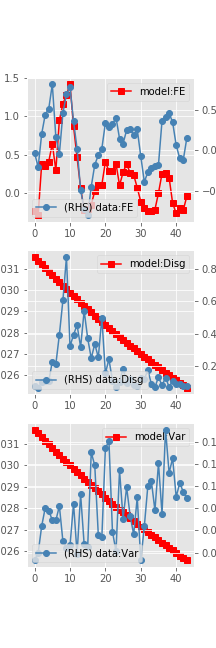
\includegraphics[width=\textwidth, height = 0.8\textheight]{figuresDraft/spf_ni_est_diag3.png}
		\end{subfigure}
		\hfill
		\begin{subfigure}[b]{0.19\textwidth}
			\caption{FE/var/Disg}
			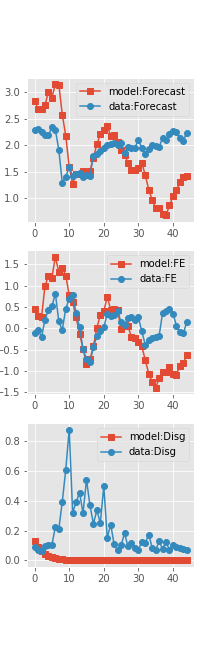
\includegraphics[width=\textwidth, height = 0.8\textheight]{figuresDraft/spf_ni_est_diag4.png}
		\end{subfigure}
	\end{figure}
\end{frame}


\begin{frame}{Results: households and NIAR}
	\begin{figure}[ht]
		\label{NI_diag_SCE}
		\begin{subfigure}[b]{0.19\textwidth}
			\centering
			\caption{forecast}
			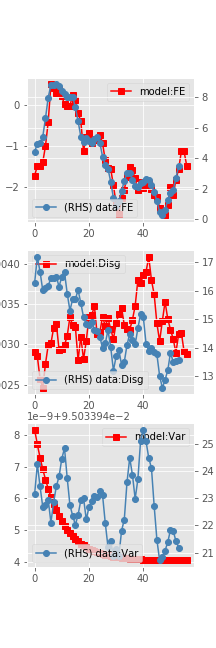
\includegraphics[width=\textwidth, height = 0.8\textheight]{figuresDraft/sce_ni_est_diag0.png}
		\end{subfigure}
		\hfill
		\begin{subfigure}[b]{0.19\textwidth}
			\caption{FE}
			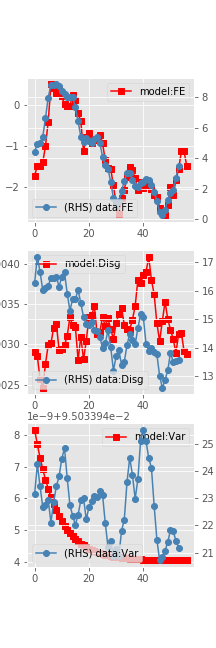
\includegraphics[width=\textwidth, height = 0.8\textheight]{figuresDraft/sce_ni_est_diag1.png}
		\end{subfigure}
		\hfill
		\begin{subfigure}[b]{0.19\textwidth}
			\caption{forecast/FE}
			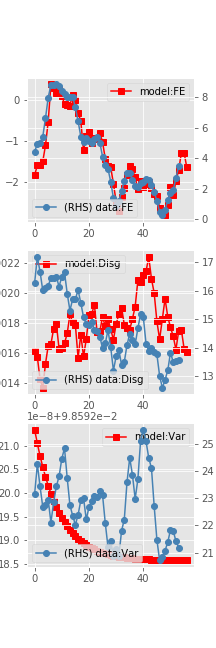
\includegraphics[width=\textwidth, height = 0.8\textheight]{figuresDraft/sce_ni_est_diag2.png}
		\end{subfigure}
		\hfill
		\begin{subfigure}[b]{0.19\textwidth}
			\caption{FE/var}
			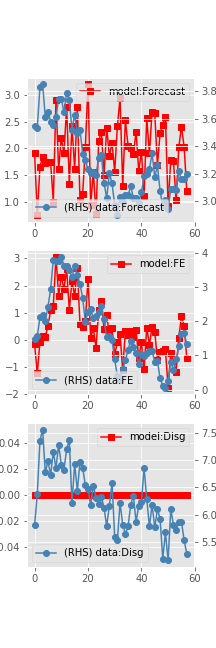
\includegraphics[width=\textwidth, height = 0.8\textheight]{figuresDraft/sce_ni_est_diag3.png}
		\end{subfigure}
		\hfill
		\begin{subfigure}[b]{0.19\textwidth}
			\caption{FE/var/Disg}
			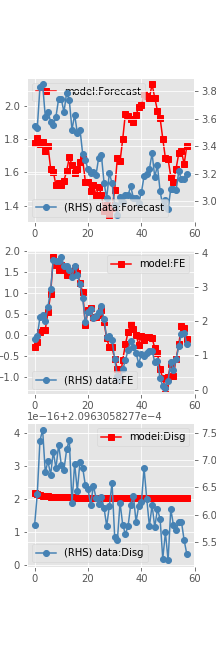
\includegraphics[width=\textwidth, height = 0.8\textheight]{figuresDraft/sce_ni_est_diag4.png}
		\end{subfigure}
	\end{figure}
\end{frame}

\begin{frame}{NIAR parameters}
	\begin{table}
		\centering
		\caption{Minimum Distance Estimates of Parameters of NI}
		\label{GMM_Est_NI_Table}
		\begin{tabular}{llllll}
	\begin{tabular}{lllllll}
		\hline 
		0        & 1    & 2   & NI: $\hat\sigma_{pb,SPF}$ & $\hat\sigma_{pr,SPF}$ & NI: $\hat\sigma_{pb,SCE}$ & $\hat\sigma_{pr,SCE}$ \\
		\hline 
		Forecast &      &     & 39.65                     & 192.22                & 2.35                      & 0.38                  \\
		FE       &      &     & 12.64                     & 211.14                & 1.64                      & 0                     \\
		FE       & Disg &     & 112.37                    & 0.34                  & 512.51                    & 0.86                  \\
		FE       & Var  &     & 1.13                      & 367.43                & 0                         & 1.28                  \\
		FE       & Disg & Var & 1.29                      & 29.84                 & 2.74                      & 127.86                \\
		\hline 
	\end{tabular}  
		\end{tabular}
	\end{table}	
\begin{itemize}
	\item $\sigma_{pb}$: noisiness of public signals in NI
	\item $\sigma_{pr}$: noisiness of private signals in Ni 
\end{itemize}
\end{frame}

\subsection{Stocastic volatility}


\begin{frame}{Results: professionals and SESV}
	\begin{figure}[ht]
		\label{SESV_diag_SPF}
		\begin{subfigure}[b]{0.19\textwidth}
			\centering
			\caption{forecast}
			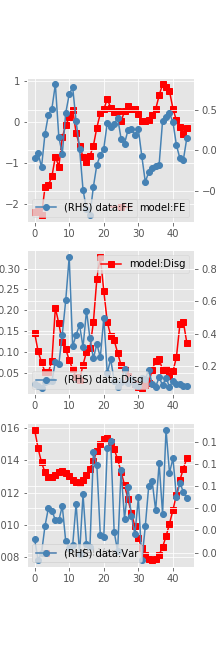
\includegraphics[width=\textwidth, height = 0.8\textheight]{figuresDraft/spf_se_est_sv_diag0.png}
		\end{subfigure}
		\hfill
		\begin{subfigure}[b]{0.19\textwidth}
			\caption{FE}
			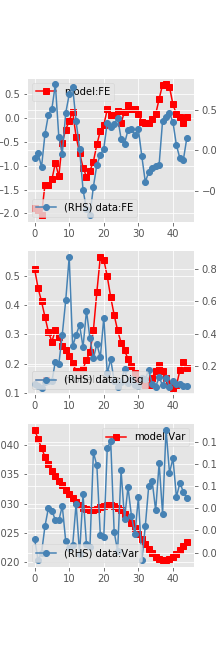
\includegraphics[width=\textwidth, height = 0.8\textheight]{figuresDraft/spf_se_est_sv_diag1.png}
		\end{subfigure}
		\hfill
		\begin{subfigure}[b]{0.19\textwidth}
			\caption{forecast/FE}
			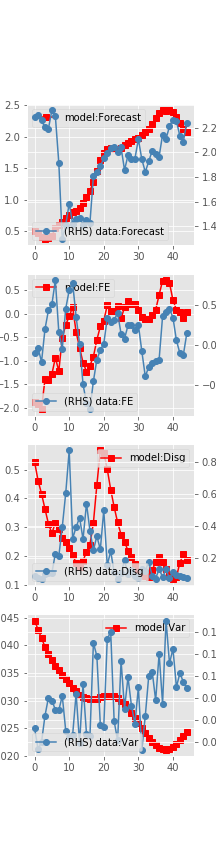
\includegraphics[width=\textwidth, height = 0.8\textheight]{figuresDraft/spf_se_est_sv_diag2.png}
		\end{subfigure}
		\hfill
		\begin{subfigure}[b]{0.19\textwidth}
			\caption{FE/var}
			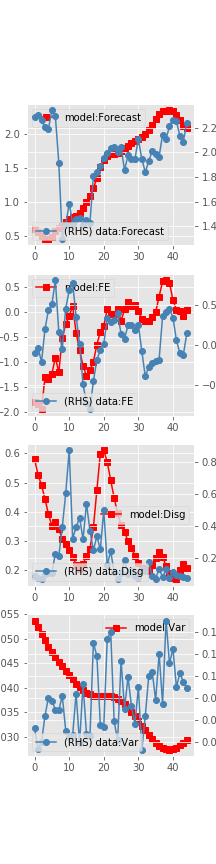
\includegraphics[width=\textwidth, height = 0.8\textheight]{figuresDraft/spf_se_est_sv_diag3.png}
		\end{subfigure}
		\hfill
		\begin{subfigure}[b]{0.19\textwidth}
			\caption{FE/var/Disg}
			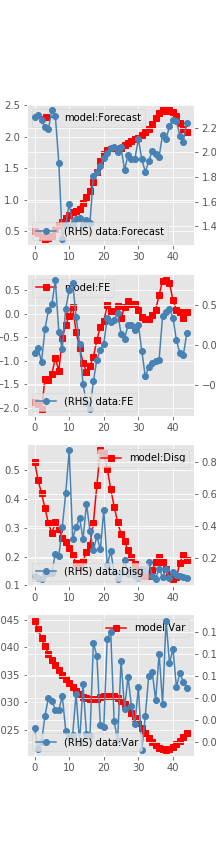
\includegraphics[width=\textwidth, height = 0.8\textheight]{figuresDraft/spf_se_est_sv_diag4.png}
		\end{subfigure}
	\end{figure}
\end{frame}


\begin{frame}{Results: households and SESV}
	\begin{figure}[ht]
		\label{SESV_diag_SCE}
		\begin{subfigure}[b]{0.19\textwidth}
			\centering
			\caption{forecast}
			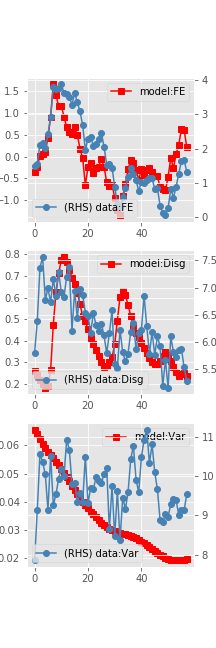
\includegraphics[width=\textwidth, height = 0.8\textheight]{figuresDraft/sce_se_est_sv_diag0.png}
		\end{subfigure}
		\hfill
		\begin{subfigure}[b]{0.19\textwidth}
			\caption{FE}
			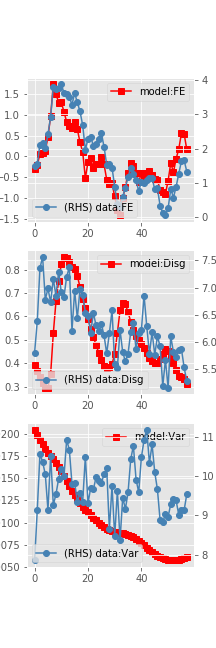
\includegraphics[width=\textwidth, height = 0.8\textheight]{figuresDraft/sce_se_est_sv_diag1.png}
		\end{subfigure}
		\hfill
		\begin{subfigure}[b]{0.19\textwidth}
			\caption{forecast/FE}
			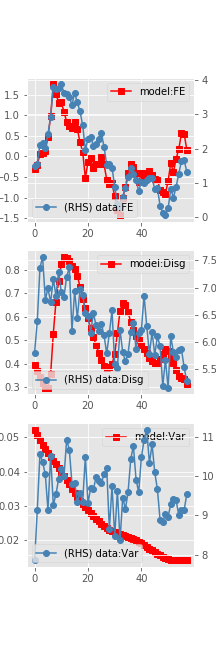
\includegraphics[width=\textwidth, height = 0.8\textheight]{figuresDraft/sce_se_est_sv_diag2.png}
		\end{subfigure}
		\hfill
		\begin{subfigure}[b]{0.19\textwidth}
			\caption{FE/var}
			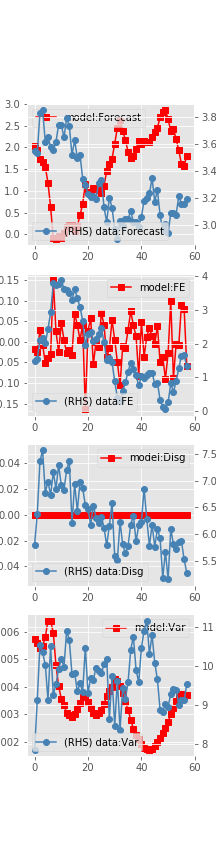
\includegraphics[width=\textwidth, height = 0.8\textheight]{figuresDraft/sce_se_est_sv_diag3.png}
		\end{subfigure}
		\hfill
		\begin{subfigure}[b]{0.19\textwidth}
			\caption{FE/var/Disg}
			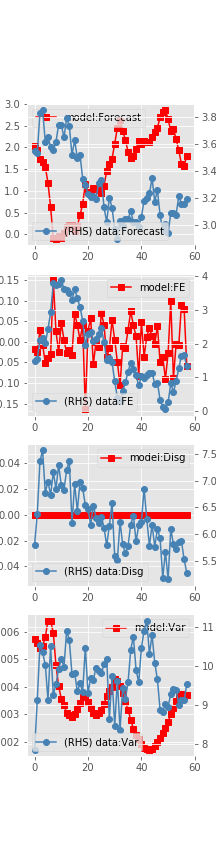
\includegraphics[width=\textwidth, height = 0.8\textheight]{figuresDraft/sce_se_est_sv_diag4.png}
		\end{subfigure}
	\end{figure}
\end{frame}



\begin{frame}{SESV parameters}
	\begin{table}
		\centering
		\caption{Minimum Distance Estimates of Parameters of SESV}
		\label{GMM_Est_SE_SV_Table}
	\begin{tabular}{lllll}
		\hline 
		0        & 1    & 2   & SE: $\hat\lambda_{SPF}$(Q) & SE: $\hat\lambda_{SCE}$(M) \\
			\hline 
		Forecast &      &     & 0.1                        & 0.02                       \\
		FE       &      &     & 0.12                       & 1                          \\
		FE       & Disg &     & 0.14                       & 1                          \\
		FE       & Var  &     & 0.12                       & 1                          \\
		FE       & Disg & Var & 0.14                       & 1                         \\
			\hline 
	\end{tabular}
\begin{itemize}
	\item $\lambda$: update rate in SE
\end{itemize}
	\end{table}	
\end{frame}


\begin{frame}{Results: professionals and NISV}
	\begin{figure}[ht]
		\label{NISV_diag_SPF}
		\begin{subfigure}[b]{0.19\textwidth}
			\centering
			\caption{forecast}
			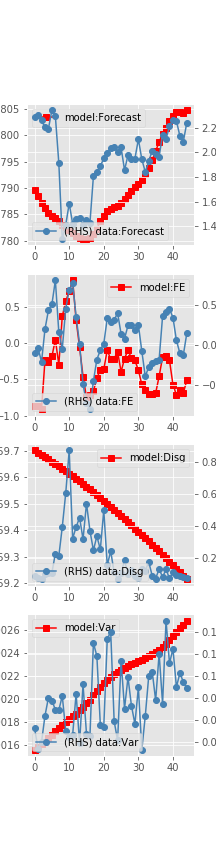
\includegraphics[width=\textwidth, height = 0.8\textheight]{figuresDraft/spf_ni_est_sv_diag0.png}
		\end{subfigure}
		\hfill
		\begin{subfigure}[b]{0.19\textwidth}
			\caption{FE}
			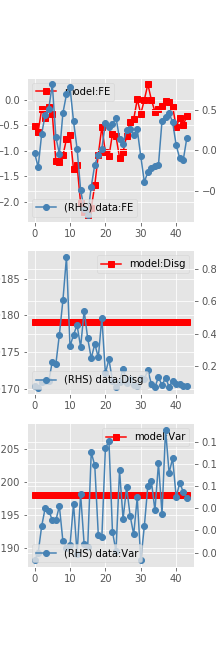
\includegraphics[width=\textwidth, height = 0.8\textheight]{figuresDraft/spf_ni_est_sv_diag1.png}
		\end{subfigure}
		\hfill
		\begin{subfigure}[b]{0.19\textwidth}
			\caption{forecast/FE}
			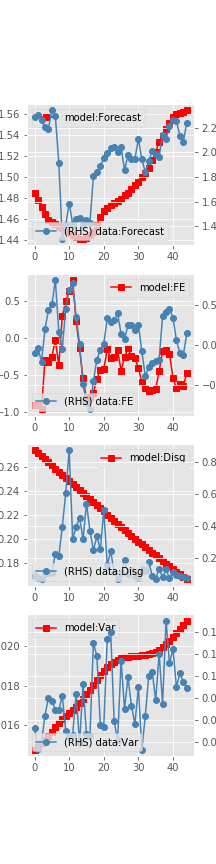
\includegraphics[width=\textwidth, height = 0.8\textheight]{figuresDraft/spf_ni_est_sv_diag2.png}
		\end{subfigure}
		\hfill
		\begin{subfigure}[b]{0.19\textwidth}
			\caption{FE/var}
			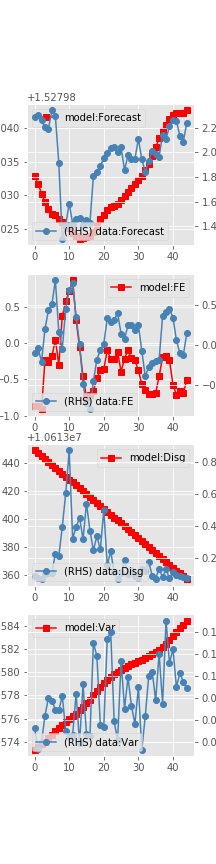
\includegraphics[width=\textwidth, height = 0.8\textheight]{figuresDraft/spf_ni_est_sv_diag3.png}
		\end{subfigure}
		\hfill
		\begin{subfigure}[b]{0.19\textwidth}
			\caption{FE/var/Disg}
			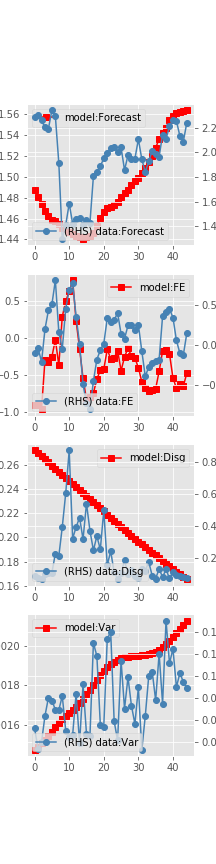
\includegraphics[width=\textwidth, height = 0.8\textheight]{figuresDraft/spf_ni_est_sv_diag4.png}
		\end{subfigure}
	\end{figure}
\end{frame}


\begin{frame}{Results: households and NISV}
	\begin{figure}[ht]
		\label{NISV_diag_SCE}
		\begin{subfigure}[b]{0.19\textwidth}
			\centering
			\caption{forecast}
			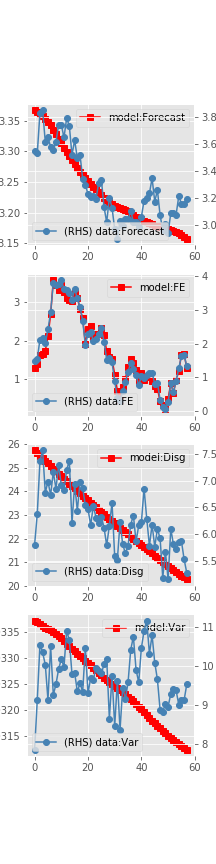
\includegraphics[width=\textwidth, height = 0.8\textheight]{figuresDraft/sce_ni_est_sv_diag0.png}
		\end{subfigure}
		\hfill
		\begin{subfigure}[b]{0.19\textwidth}
			\caption{FE}
			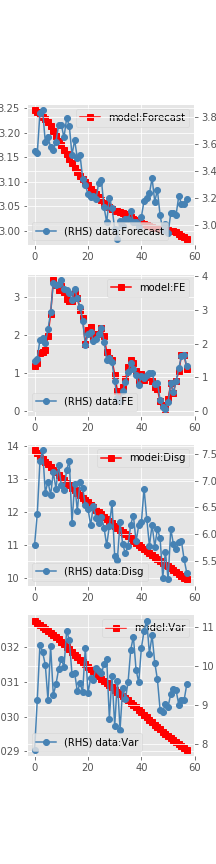
\includegraphics[width=\textwidth, height = 0.8\textheight]{figuresDraft/sce_ni_est_sv_diag1.png}
		\end{subfigure}
		\hfill
		\begin{subfigure}[b]{0.19\textwidth}
			\caption{forecast/FE}
			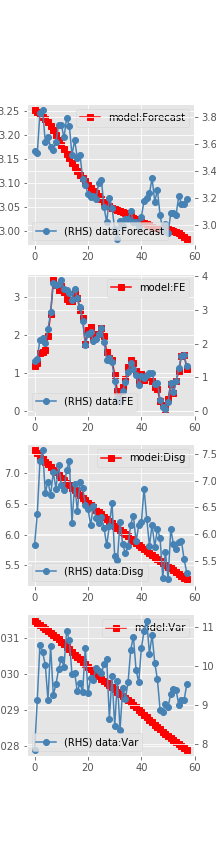
\includegraphics[width=\textwidth, height = 0.8\textheight]{figuresDraft/sce_ni_est_sv_diag2.png}
		\end{subfigure}
		\hfill
		\begin{subfigure}[b]{0.19\textwidth}
			\caption{FE/var}
			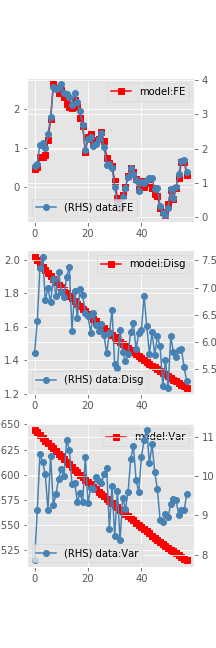
\includegraphics[width=\textwidth, height = 0.8\textheight]{figuresDraft/sce_ni_est_sv_diag3.png}
		\end{subfigure}
		\hfill
		\begin{subfigure}[b]{0.19\textwidth}
			\caption{FE/var/Disg}
			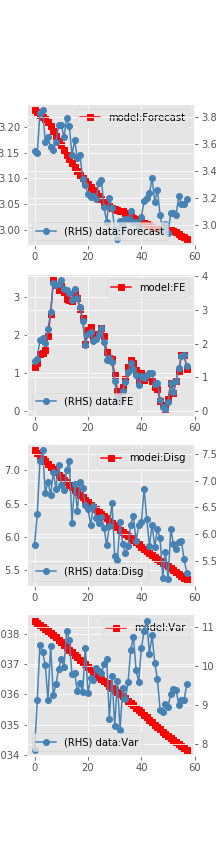
\includegraphics[width=\textwidth, height = 0.8\textheight]{figuresDraft/sce_ni_est_sv_diag4.png}
		\end{subfigure}
	\end{figure}
\end{frame}


\begin{frame}{NISV parameters}
	\begin{table}
		\centering
		\caption{Minimum Distance Estimates of Parameters of NISV}
		\label{GMM_Est_NI_SV_Table}
	\begin{tabular}{lllllll}
		\hline 
		0        & 1    & 2   & NI: $\hat\sigma_{pb,SPF}$ & $\hat\sigma_{pr,SPF}$ & NI: $\hat\sigma_{pb,SCE}$ & $\hat\sigma_{pr,SCE}$ \\
		\hline 
		Forecast &      &     & 16.9                      & 21.44                 & 5.21                      & 6.05                  \\
		FE       &      &     & 67.05                     & 146.8                 & 4.4                       & 4.88                  \\
		FE       & Disg &     & 62.6                      & 0.57                  & 7.23                      & 3.54                  \\
		FE       & Var  &     & 787.17                    & 3257.84               & 97.72                     & 95.73                 \\
		FE       & Disg & Var & 126.68                    & 0.57                  & 215.54                    & 3.64                 \\
		\hline 
	\end{tabular}
	\end{table}	
\begin{itemize}
	\item $\sigma_{pb}$: noisiness of public signals in NI
	\item $\sigma_{pr}$: noisiness of private signals in NI 
\end{itemize}
\end{frame}


\begin{frame}{Ongoing work}
	\begin{itemize}
		\item I have been matching time-specific conditional moments with data. I will match unconditional moments
		\item jointly estimate process parameters and expectation formation parameters
		\item statistical tests of the fitness,  i.e. Sargan–Hansen test in the GMM
	\end{itemize}	
\end{frame}

\section{Conclusion}

\begin{frame}{Conclusion}
	\begin{itemize}
		\item Sticky expectation (SE) matches data of inflation and expectations better compared to noisy information (NI) 
		\item Within each model,  households are more irrational compared to professionals
		\item Incorporating higher moments, i.e. uncertainty,  helps ``discipline'' theories on expectation formation
		\item  Higher moments from surveys also contain useful information about the inflation dynamics itself
	\end{itemize}	
\end{frame}

\bibliographystyle{apalike}
\bibliography{ExpSlides}


\end{document}
